\chapter{RESULTADOS E DISCUSSÃO}

Entender como a contribuição acadêmica influencia na intenção inicial da carreira empreendedora é de grande interesse para centros acadêmicos, profissionais e educadores em empreendedorismo. Desta forma os resultados desta pesquisa encontram-se divididos em seções, que atendem aos objetivos propostos no estudo.
Inicialmente são apresentadas descrições que caracterizam os dois perfis estudados
(pré-programa e pós-programa) em relação às variáveis e as comparações entre os grupos. Posteriormente serão apresentadas as inovações produzidas pelos alunos participantes durante o decorrer do programa.



\section{Materiais de apoio para desenvolvimento do aprendizado teórico dos conteúdos: Aplicativo Empreenda Agro Sustentável}



Muitos aplicativos móveis agrícolas pagos e gratuitos foram desenvolvidos para o meio rural, abrangendo diversas áreas dentro e fora da propriedade rural \cite{silva_environment_2015}. A tecnologia da informação apresenta grandes potencialidades para auxiliar produtores rurais e profissionais da área na tomada de decisões estratégicas. Todavia, para o profissional das ciências agrárias tomar decisões assertivas, não basta apenas manusear a Tecnologia da Informação aplicada ao agronegócio, é   necessário   mudar   a   concepção   dos   processos   a   partir   de   sua informatização \cite{ferraz_tecnologia_2017}.

A área de edtech no Brasil segue em franco crescimento. Segundo relatório da \citeonline{abstartups_mapeamento_2020} o país conta com 449 Startups focadas em aplicação sistemática de conhecimento científico para tarefas práticas, das quais 48,11/\% são direcionadas ao ensino superior, o aplicativo Empreenda Agro, se soma a estas ferramentas, ele foi desenvolvido para ser ferramenta portátil, acessível e utilizável por acadêmicos das Ciências Agrárias no sentido de dar direcionamento educacional em empreendedorismo. 


\subsection{Recursos e funcionalidades do aplicativo}

O aplicativo consiste em uma interface com bancos de dados que permite ao usuário averiguar, de modo interativo, os conteúdos melhor recomendados para o aprendizado da cultura empreendedora para as áreas das ciências agrárias. 

Para o acesso de dados através do dispositivo portátil, o mesmo pode ser instalado com apenas alguns cliques, onde o usuário não precisa estar inscrito ou participando do programa, para efetuar o primeiro acesso. É necessário apenas ter disponibilidade de rede de internet local ou móvel, que permita o primeiro download das informações. Após concluir a transmissão de dados para o aplicativo, não se faz necessário ter continuidade da Internet para utilizar o aplicativo.

Durante a execução do aplicativo, tem-se a tela de inicialização que conta com a marca do programa e aplicativo homônimo (Figura \ref{figura_42} \textcolor{blue}{(a)}). 
Após, apresenta-se a tela principal (Figura \ref{figura_42} \textcolor{blue}{(b)}) do aplicativo que exibe uma lista de botões para selecionar o tipo de conteúdo de interesse do usuário. Estas funcionalidades podem ser acessadas por um menu lateral deslizante \textit{Drawer list} (Figura \ref{figura_42} \textcolor{blue}{(c)}), facilitando assim o manuseio do aplicativo pelo usuário final. 


\begin{figure}[H]
\FloatBarrier
\center
\caption{\textbf{Aplicativo Empreenda Agro Sustentável}}
\subfigure[ref1][Tela inicial]{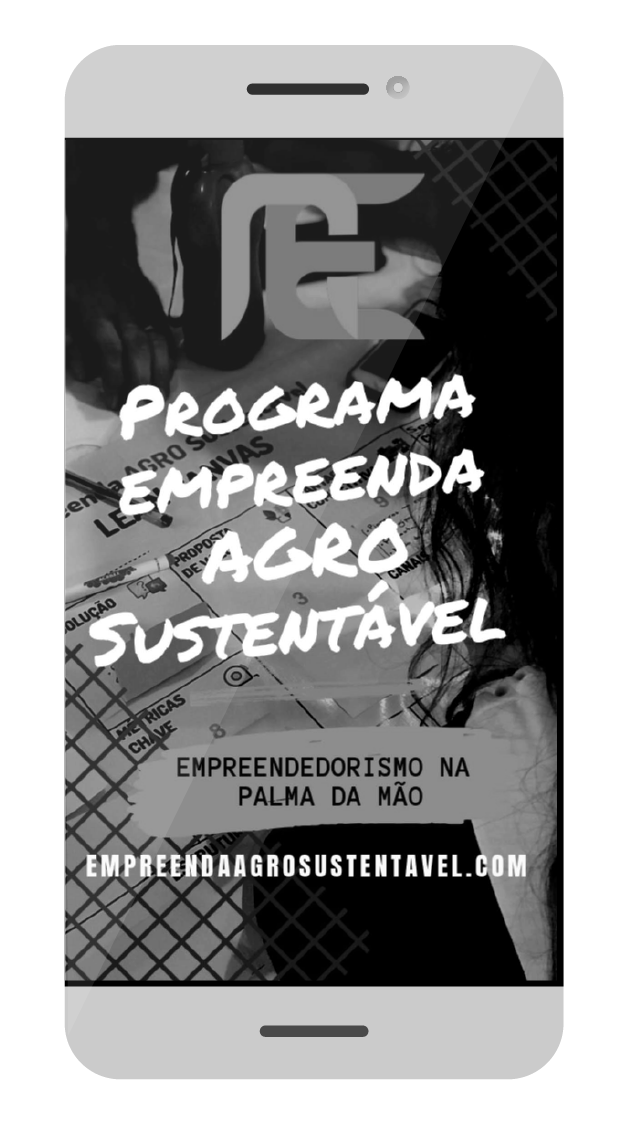
\includegraphics[scale=0.2]{Imagens/aplicativo_login.png}}
\qquad
\subfigure[ref2][Tela Principal]{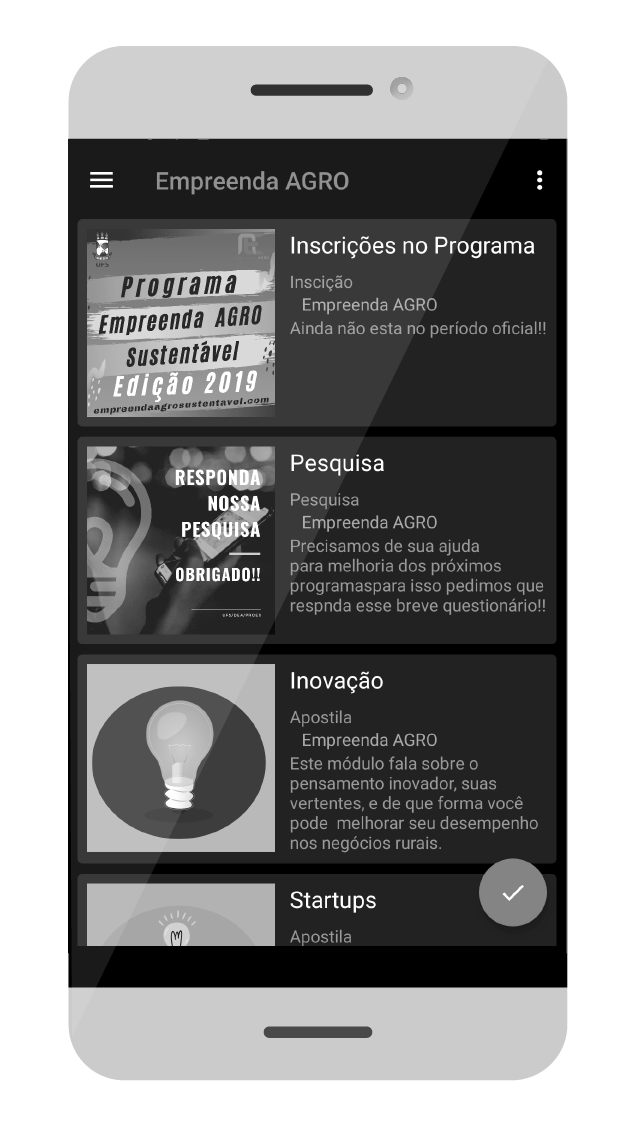
\includegraphics[scale=0.2]{Imagens/aplicativo_1.png}}
\qquad
\subfigure[ref3][\textit{Drawer list}]{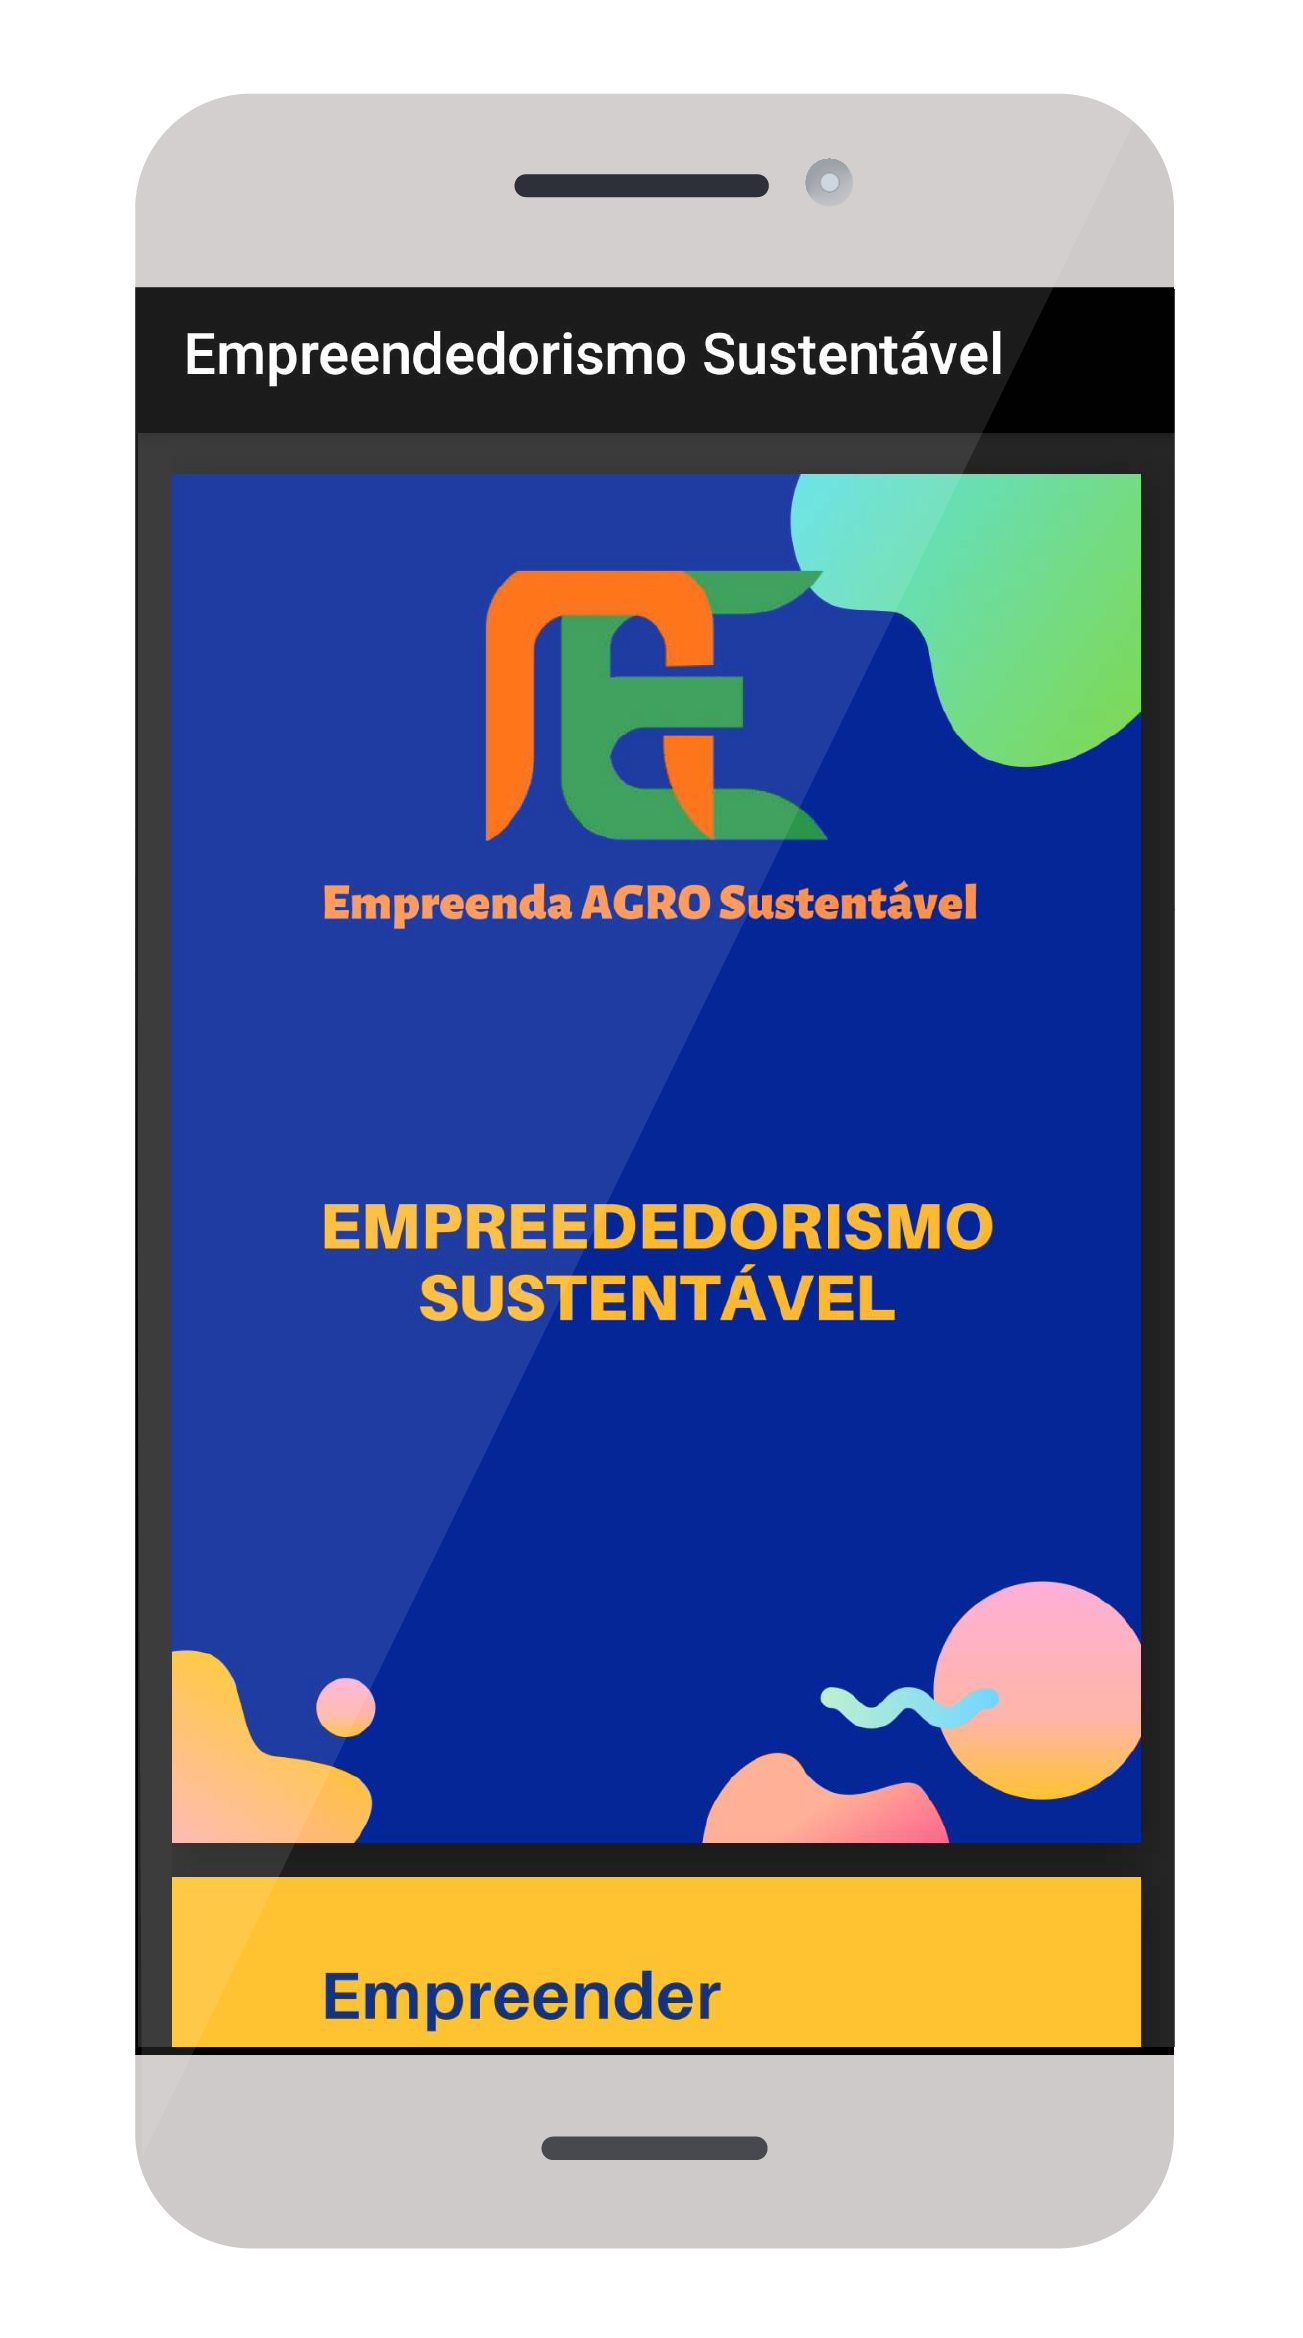
\includegraphics[scale=0.2]{Imagens/aplicativo_3.png}}
\fonte{O Autor}.
\label{figura_42}
\end{figure}
 


Todas as informações sobre o software assim como o sobre os conteúdos de apoio a serem abordados estão disponíveis, em todos os tipos de mídias (áudio, vídeo e escrito), já que o aplicativo conta com diversos formatos de mídias digitais e links com outros canais de divulgação como exemplo: O streaming Spotify (Figura \ref{figura_44} \textcolor{blue}{(a)}), o Youtube.com e o site de notícias sobre empreendedorismo Exame \ref{figura_44}a).  Para os dados escritos, o usuário poderá exportar em formato .pdf dos dados presentes no dispositivo portátil (Figura \ref{figura_44} \textcolor{blue}{(c)}).

Estas funcionalidades podem ser acessadas pelo menu lateral deslizante chamado de \textit{Drawer list} (Figura \ref{figura_42}c), facilitando assim o manuseio do aplicativo pelo usuário final. 

\begin{figure}[H]
\FloatBarrier
\center
\caption{\textbf{Aplicativo Empreenda Agro Sustentável}}
\subfigure[ref4][Podcasts]{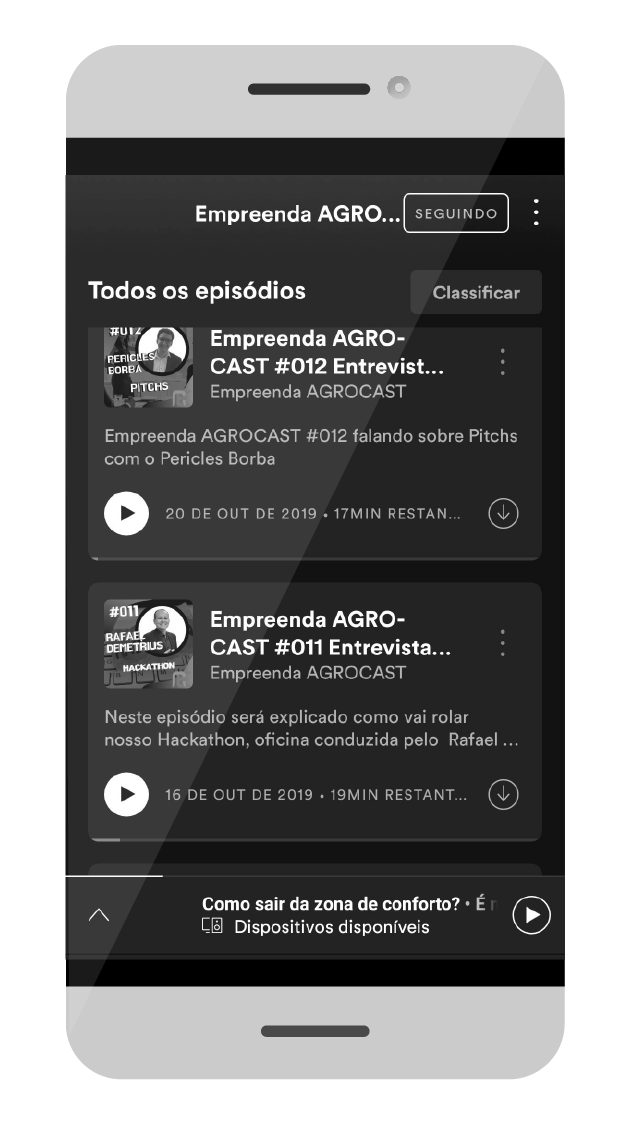
\includegraphics[scale=0.2]{Imagens/aplicativo_4.png}}
\qquad
\subfigure[ref4][Notícias sobre empreendedorismo]{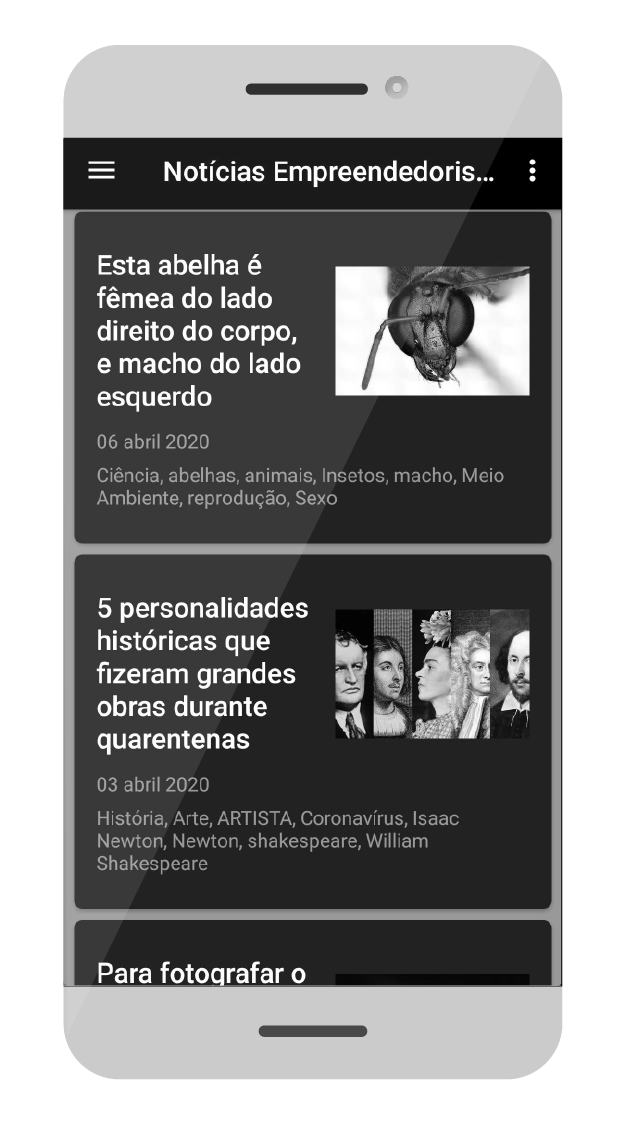
\includegraphics[scale=0.2]{Imagens/aplicativo_5.png}}
\qquad
\subfigure[ref4][Conteúdos escritos]{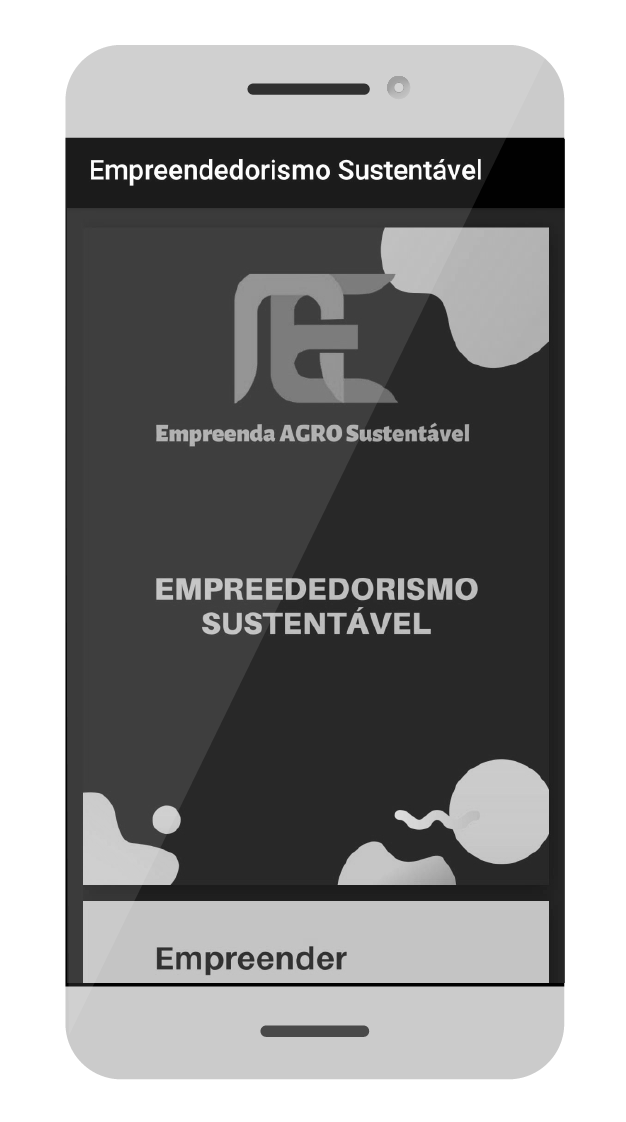
\includegraphics[scale=0.2]{Imagens/aplicativo_6.png}}
\fonte{O Autor}.
\label{figura_44}
\end{figure}


\subsection{Teste de usabilidade do aplicativo}

Os principais critérios de inclusão para os usuários testadores foi ter um telefone smartphone, pois o aplicativo foi desenvolvido apenas em uma plataforma Android, O download do aplicativo foi disponibilizado de forma grátis por meio da loja de aplicativos Google Play.

Na Figura \ref{figura_43} é possível ver a serie temporal dos downloads ao aplicativo por meio da plataforma Google Play. A maior quantidade de versões operacionais do sistema Android foi a versão 9.0 tendo alcançando 32 aparelhos ativos desde o início do lançamento (Figura \ref{figura_43}).

\begin{figure}[H]
\caption{\textbf{Série temporal dos dispositivos ativos desde o lançamento no dia 01 de outubro de 2019 até o mês de abril de 2020.}}
\centering
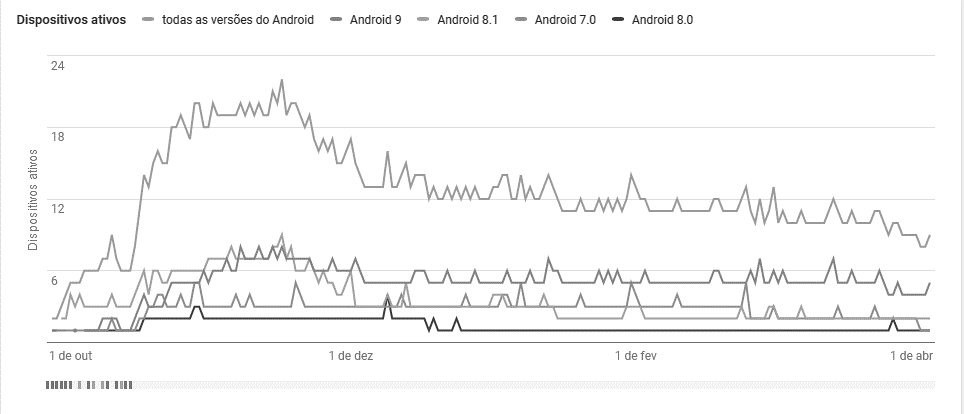
\includegraphics[scale=0.6]{Imagens/dispositivos_instalados.png}
\fonte{ \citeonline{google_developer_google_2020}}
\label{figura_43}
\end{figure}

Para o fluxo de atividade da aplicação, foi deixado aos usuários a manipulação de forma orgânica dos conteúdos, a fim de que fosse possível observar eventuais falhas durante o uso e requisição de conteúdos da plataforma. 
As tarefas específicas dos testadores de aplicativos incluíram o acesso a abas, abertura de links resultantes de dados externos; leitura fluida dos materiais disponíveis em pdf, acesso livre aos conteúdos disponíveis em vídeos, (nenhum limite foi definido para a quantidade de dados a serem registrados no aplicativo) e a navegação geral do aplicativo, de forma fluida e rápida.

Qualquer falha de acesso aos dados ou tempo de atraso na resposta do aplicativo durante o lançamento e o uso, “troca de tela”, usando o teclado deslizante e os botões da tela de toque dos aplicativos também foram monitorados, seguiram procedimentos de feedback por meio da plataforma Google Play Console, os procedimentos utilizados para teste do aplicativo foram os mesmos descritos \citeonline{adu_development_2020}.

O APP Empreenda Agro Sustentável é um aplicativo desenvolvido pelo programa, com o propósito de auxiliar os alunos dos cursos de ciências agrárias participantes ao aprendizado da educação empreendedora por meio de conteúdos dinâmicos e direcionados a área de negócios no meio rural, tais como: Materiais informativos, Vídeo aulas e podcasts.

O aplicativo também é indicado para profissionais que tenham interesse em aprender mais sobre o desenvolvimento de negócios sustentáveis e escaláveis.

A implementação destas funcionalidades dentro do aplicativo seguiu satisfatoriamente as solicitações dos usuários,.
Buscando cumprir os requisitos de aquisição de direito e propriedade autoral o aplicativo foi registrado no Instituto Nacional de Propriedade Industrial INPI sob número de registro \textbf{BR 51 2019 002657 8} e disponível gratuitamente para testes na loja online Google Play Store, de propriedade da Universidade Promotora do Programa.

\section{Alcance da amostra experimental}

No desenvolvimento do programa foram formadas inicialmente 26 equipes que somaram 118 alunos oriundos dos cursos de graduação do Centro de Agrárias e Aplicadas além de outros cursos como: Artes Visuais, Administração, Design Gráfico, Engenharia Química, Engenharia de Produção, Marketing e Ecologia.
Os dados coletados revelam que, nas 115 respostas válidas que compõem a amostra a faixa etária no período de inscrição, apresentavam 75,4\% dos estudantes com idade menor que 20 anos, 16,1\% apresentaram a intervalo de idades entre 21 e 25 anos, e 59\% tinham idade maior que 25 anos (Tabela \ref{tabela_45}).
 
\begin{table}[H]
\centering
\caption{\textbf{Faixa etária dos alunos participantes do programa}}
\label{tabela_45}
\begin{tabular}{clcc} 
\hline\hline
 \textbf{Dados}                       & \textbf{Faixa etária}  & \multicolumn{2}{c}{~\textbf{Inscritos} }                                                        \\ 
\hline
\multirow{3}{*}{}                     &                        & \multicolumn{1}{l}{\textbf{Frequência (\%)} } & \multicolumn{1}{l}{\textbf{Porcentagem (\%)} }  \\
                                      & \textbf{Menor que 20}  & 89                                            & 75,4                                            \\
                                      & \textbf{De 21 a 25}    & 19                                            & 16,1                                            \\
\multicolumn{1}{l}{\textbf{Válidos} } & \textbf{Maior que 25}  & 7                                             & 5,9                                             \\
\multicolumn{1}{l}{}                  & \textbf{Total}         & 115                                           & 97,5                                            \\ 
\hline
\multicolumn{1}{l}{\textbf{Omissos} } & \textbf{Não informou}  & 3                                             & 2,5                                             \\ 
\hline
\multicolumn{2}{c}{\textbf{TOTAL GERAL} }                      & \multicolumn{1}{l}{118}                       &                                                 \\
\hline\hline
\end{tabular}
\fonte{O autor}
\end{table}


O curso com maior participação numérica foi o de Engenharia Agronômica, representando 47,32\% deste total, enquanto os cursos de Engenharia Agrícola, Zootecnia, Engenharia de Pesca e Engenharia Florestal participaram em termos percentuais e respectivamente com 11,61\%, 19,64\%, 4,46\% e 6,25\% do total de estudantes inscritos. Na Figura \ref{figura_10} são apresentados dados sobre a quantidade de alunos inscritos e seus respectivos cursos.



\begin{figure}[H]
\caption{\textbf{Numero de alunos inscritos e percentual por curso no universo total de participantes do Programa.}}
\centering
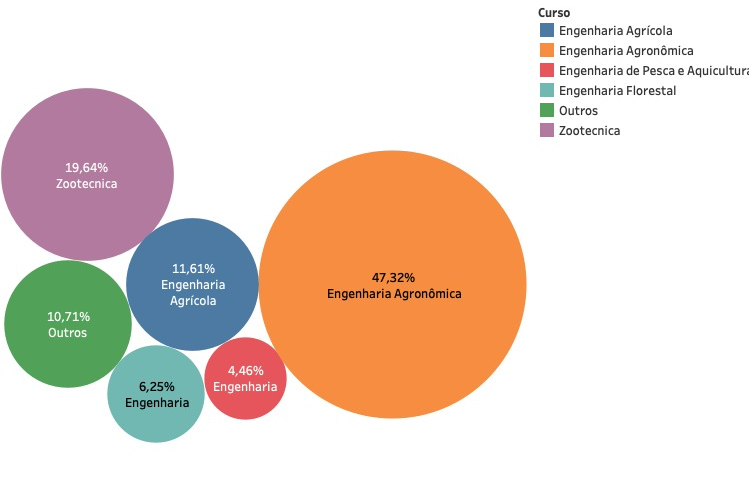
\includegraphics[scale=0.3]{Imagens/inscritos.png}
\fonte{O autor}
\label{figura_10}
\end{figure}

\section{Áreas e cadeias produtivas selecionadas}

A fase de inscrição do programa alcançou 27 propostas de protótipos e/ou negócios na área rural com foco na agricultura sustentável. Na figura \ref{figura_11} é possível verificar as áreas e cadeias produtivas prioritárias escolhidas. Das quais deram continuidades durante todo o projeto 15 equipes.

As propostas de negócios se focaram em sua maior quantidade em produtos ligados a aplicações moveis (31\%), seguido de negócios ligados a agricultura sustentável (23\%). Muitos aplicativos móveis agrícolas pagos e gratuitos foram desenvolvidos para o meio rural, abrangendo diversas áreas dentro e fora da propriedade rural \cite{silva_caracterizacao_2017}. 




\begin{figure}[H]
\centering
\caption{\textbf{Áreas e potenciais propostas de negócios escritos}}
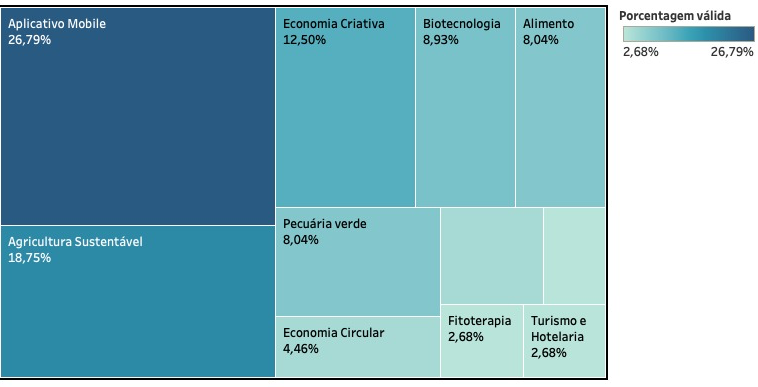
\includegraphics[scale=0.6]{Imagens/propostas_negocios.png}
\fonte{O autor}
\label{figura_11}
\end{figure}


A tecnologia da informação apresenta grandes potencialidades para auxiliar produtores rurais e profissionais da área na tomada de decisões estratégicas, de modo que, o mercado de aplicativos móveis tem tomado força no campo. . Todavia, para o profissional das ciências agrárias tomar decisões assertivas, não basta apenas manusear a Tecnologia da Informação aplicada ao agronegócio, é   necessário   mudar a concepção dos processos a partir de sua informatização \cite{ferraz_tecnologia_2017,sharma_systematic_2020}. 

Grandes desafios, como a competição de recursos, aumento populacional, competição por terras agricultáveis, representam ameaças à segurança alimentar do planeta, especialmente aos países em desenvolvimento e subdesenvolvidos \cite{pardey_bounds_2014}. 

Se mostra natural o crescimento do debate sobre a agricultura sustentável, já que o tem disso crescente as discussões sobre o paradigma crescimento da produção de forma sustentável, 
\citeonline{rockstrom_sustainable_2017} argumentam que, que esse paradigma deve ser definido em todas as escalas no contexto atual que vivemos de rápidas mudanças ambientais, globais no Antropoceno, ao mesmo tem que deve a agricultura também deve se concentrar na erradicação da pobreza e da fome e contribui para o bem-estar humano.

Buscando mitigar este problemas cada vez mais complexos na produção agrícola, os avanços na agricultura inteligente, métodos de tomada de decisão balizada nas técnicas de informação,  agricultura de precisão, e novas tecnologias embarcadas, oferecem ferramentas importantes para enfrentar estes desafios, mantendo a sustentabilidade agrícola, já que as práticas agrícolas não se concentram apenas no enriquecimento da produtividade agrícola, mas também ajudam a reduzir impactos ambientais prejudiciais de forma sustentável \cite{adnan_effects_2018,rockstrom_sustainable_2017,ye_bio-organic_2020}. 


\section{Contextualizando o cenário da prática}

Para a uniformização da linguagem e terminologias tratadas nesse artigo, de agora em diante, não mais faremos referência ás “oficinas”, que substituímos por “Workshops”, uma vez que foi essa a terminologia utilizada nos textos do projeto submetido á PROEX/UFS, assim como em todo material de divulgação. 

Os encontros com os alunos aconteceram mensalmente, de maneira presencial durante dois dias em dois turnos. A proposta da metodologia contemplou a divulgação semanal de atividades desenvolvidas pelos grupos, a fim de manter o engajamento dos participantes e desenvolvimento das propostas de negócios pensadas ao entrarem no programa. Inicialmente, foi desenvolvido um site \href{http://www.empreendaagrosustentavel.com}{empreendaagroustentavel.com}  para divulgação do programa proposto. A cada Workshop, foram desenvolvidas atividades práticas, obedecendo aos seguintes critérios: Desenvolvimento gradual da ideia de negócio de forma planejada; Desenvolvimento de planos de negócios e planos gerenciais; Desenvolvimento do mínimo produto economicamente viável; Aprendizado e estratégia de apresentação do produto proposto.
 

O indivíduo é o conjunto de seus Conhecimentos, Habilidades e Atitudes (CHA) \cite{dutra_competencias_2004}, conjunto este de grande relevância para um empreendedor, especialmente porque as competências se mostram como parte fundamental da formação do empreendedor nos dias atuais, o qual assume a responsabilidade de agregar valor às organizações \cite{ferreira_conhecimento_2019}, desta forma, se mostra importante o aprendizado contínuo e multidisciplinar para fixação e melhor desenvolvimento dos conteúdos aprendidos. \citeonline{limberger_metodologias_2013} ressalta que, as metodologias ativas proporcionam uma visão reflexiva maior que a apresentada nos métodos tradicionais de ensino: 

\begin{citacao}
[...] Quando o aprendizado ocorre por meio de metodologias ativas, o conhecimento dos estudantes é comparável ao do método tradicional, porém, seu desempenho em relação às suas habilidades e atitudes é superior, reflexo da visão crítico reflexiva proporcionada pelo método.[...] \cite{limberger_metodologias_2013}.
\end{citacao}


Foram promovidos quatro Workshops, nos quais foram abordados, os conceitos de empreendedorismo, ideação, modelo de negócios, marketing, entre outros. As oficinas foram conduzidas através de palestras, a    tividades práticas e dinâmicas, ou seja, metodologias ativas. Os Workshops foram conduzidos no formato de “Jornada” (Figura \ref{figura_17}), ou seja, aos participantes foram apresentados gradativamente a conteúdos e metodologias. 


\begin{figure}[H]
\centering
\caption{\textbf{Jornada Empreenda Agro Sustentável}}
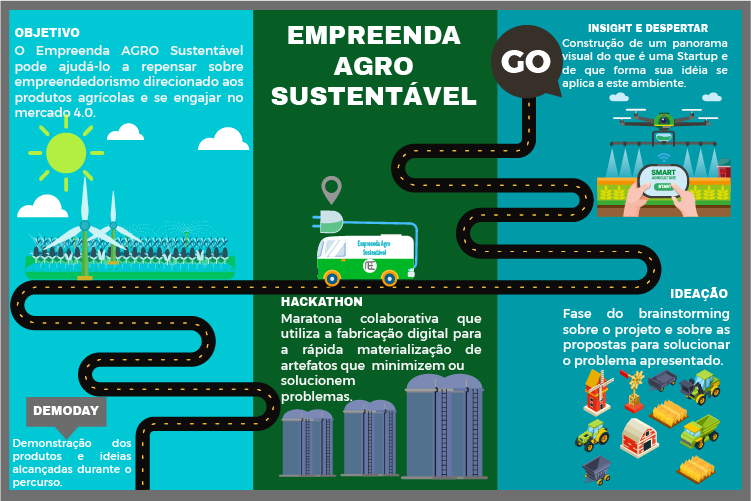
\includegraphics[scale=0.5]{Imagens/jornada.png}
\fonte{O autor}
\label{figura_17}
\end{figure}


Numa sequência encadeada de conteúdos e práticas as equipes formadas, e sempre numa dinâmica proativa, iniciaram a jornada com o “despertar”, que já acontecia antes mesmo da realização do primeiro Workshop, por meio das várias intervenções ainda usando formas remotas de comunicação, que repassaram conteúdo a partir de materiais escritos e  podcasts disponibilizados no site do programa \href{https://open.spotify.com/show/3c25hRSxvaCFPw6Y3lX3i1?si=9H_fGz_uRgGiFNhAcdr4rQ}{Empreenda AGROCAST} (Apêndice \ref{app:poscast}. 

Orientados pela jornada posta, as equipes foram reunidas para o Workshop inicial em que a etapa do “despertar” ganhava voz, já oportunizando os momentos inicias da “ideação”. Na sequência de Workshops em que o processo de ideação foi evoluindo, com tempo para possível pivotagem, foi então alcançada a etapa   de “prototipagem” da jornada. Como etapa final foi então realizado o “Demoday”, em que as equipes apresentaram os seus pitchs, para investidores, concluindo uma jornada com duração de 6 meses.


\subsection{Primeiro Workshop}

As atividades foram iniciadas com a abertura do programa feita pela equipe organizadora, na qual foi apresentada a programação dos Workshops, denominada de “A Jornada”. O momento do programa (1º Workshop) teve como foco o desenvolvimento de palestras e oficinas que abordaram temas relacionados ao empreendedorismo, tais como: Startups, Empreendedorismo, comportamento empreendedor e cultura empreendedora, Problemas (segmentação do mercado) segundo as ODS (Objetivos do Desenvolvimento Sustentável) (Figura \ref{fig:ods}) e Agritechs na palestra “Tecnologias digitais e as oportunidades para o Agronegócio”. Como prática tendo como base pedagógica as metodologias ativas, teve o início do desenvolvimento do Lean Canvas, com foco no bloco referente a proposta de valor, imagens das atividades podem ser vistas no Apêndice \ref{app:workshop_1}.

\begin{figure}[H]
\centering
\caption{\textbf{Objetivos do Desenvolvimento Sustentável - ODS}}
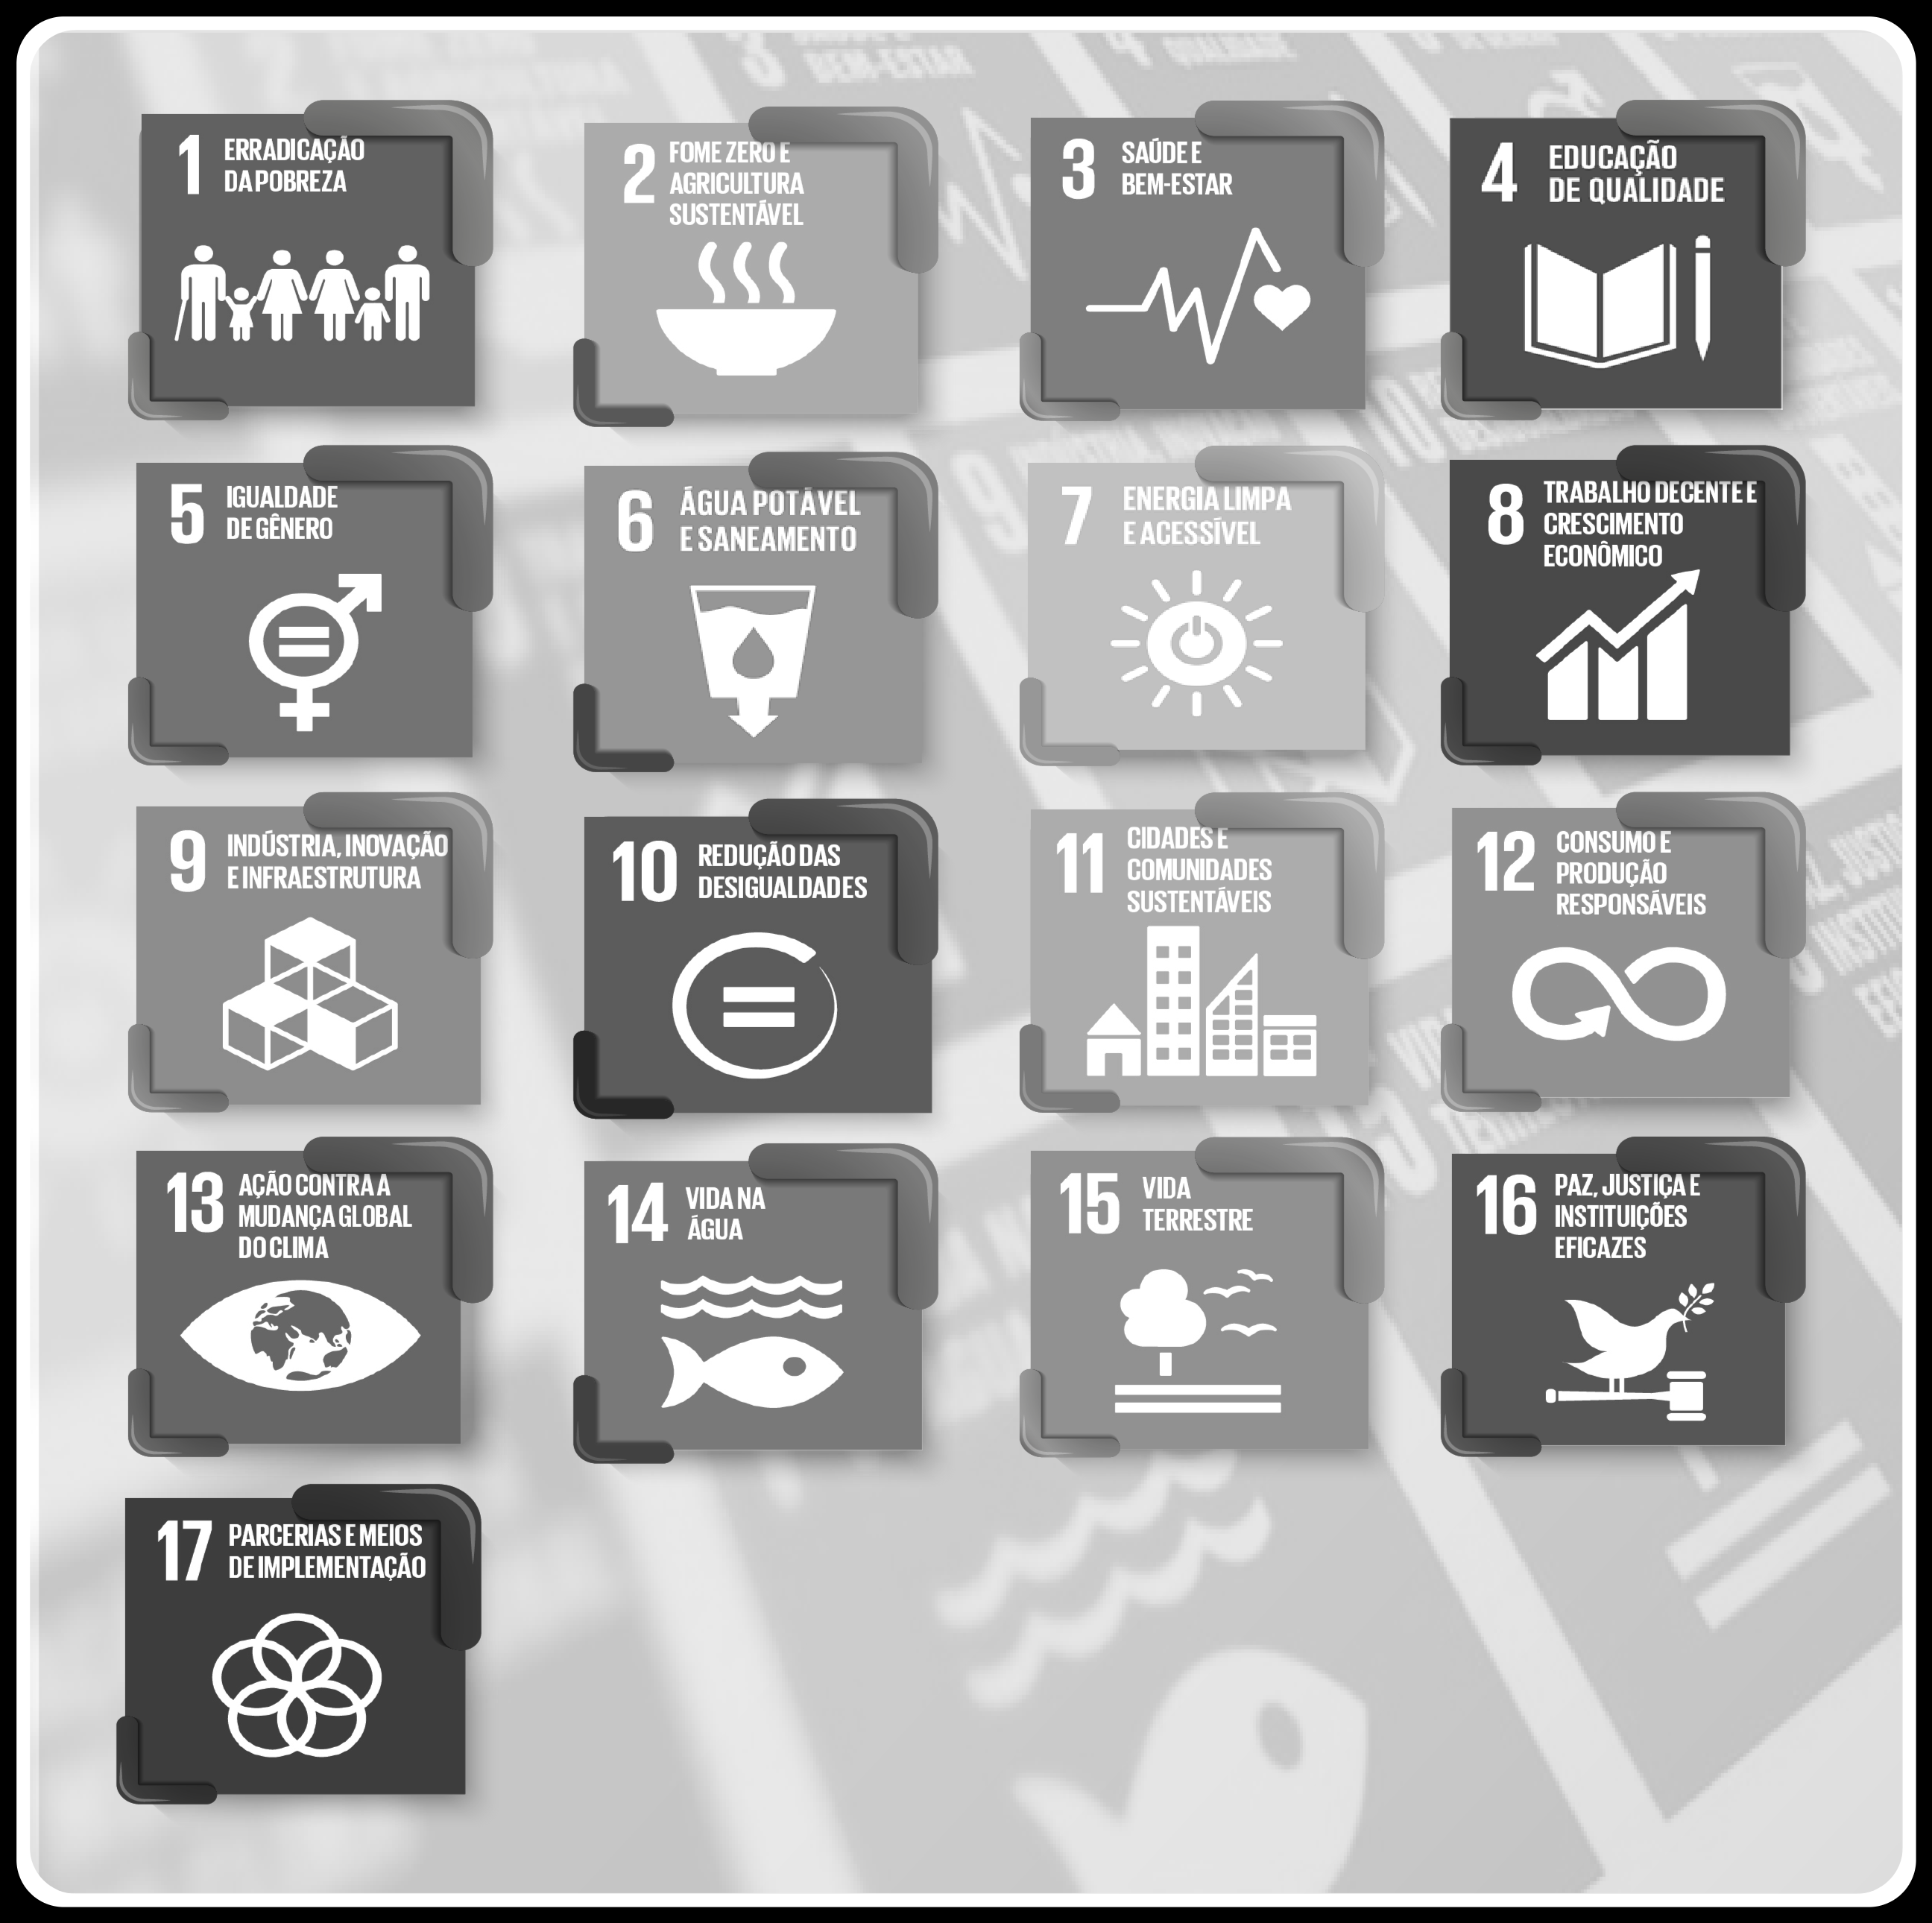
\includegraphics[scale=0.1]{Imagens/ODS_GERAL.png}
\fonte{Adaptado de \cite{onu_agenda_2015}}
\label{fig:ods}
\end{figure}


\subsection{Segundo Workshop}


O segundo Workshop ocorreu nos dias 30 e 31 de agosto de 2019, quando foram abordados temas como a busca de oportunidades como característica fundamental de um empreendedor, economia colaborativa, \textit{coworking} e os benefícios do espaço compartilhado. Esses foram temas transversais que contribuíram para suporte teórico das equipes. De forma proativa foram aprofundados os conhecimentos sobre cada bloco do Lean Canvas (solução, canais, métricas-chave, vantagem competitiva, receitas, custos, e o fechamento da proposta de valor). 

Esses blocos foram trabalhados de forma dinâmica, possibilitando aos participantes avanços no processo de ideação que vinha sendo trabalhado pelos grupos, na formatação do modelo de negócio pretendidos. No Apêndice \ref{app:workshop_2}  (Figura \ref{figura_29}), 
e possível observar o cenário da pratica do Workshop.
 

\begin{figure}[H]
\centering
\caption{\textbf{Banner divulgação Segundo Workshop}}
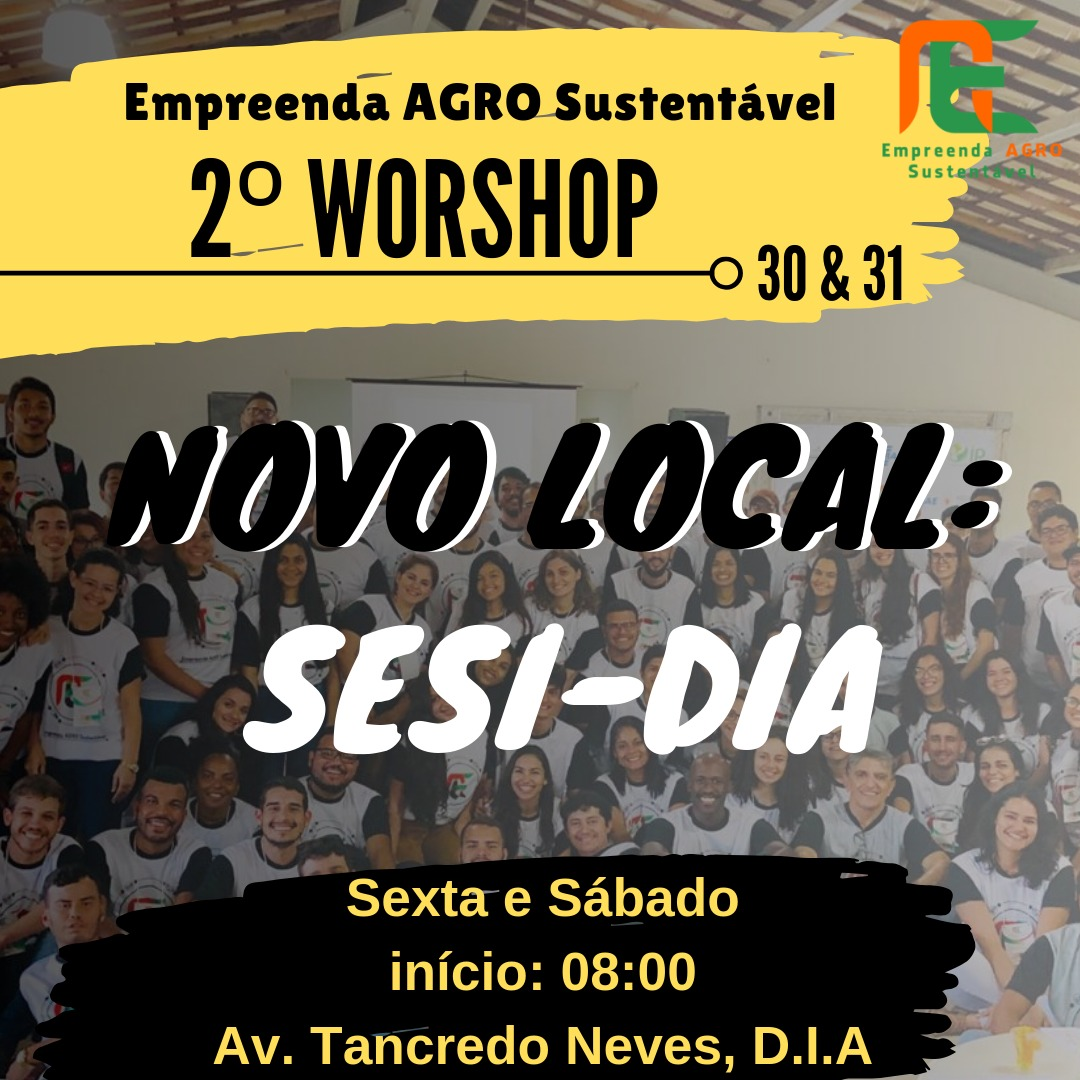
\includegraphics[scale=0.23]{Imagens/2_workshop.jpg}
\fonte{O autor}
\label{fig:ods}
\end{figure}

\subsection{Hackathon}

O terceiro Workshop foi realizado nos dias 18 e 19 de outubro de 2019. Esse Workshop foi conduzido no formato de Hackathon quando foi trabalhada a percepção do mercado, o mapa do cliente assim como a construção de protótipos, \textit{storyboard} e \textit{storytelling}. Em tempo, o Hackeaton consiste em uma maratona de programação, na qual as equipes tiveram a oportunidade de trabalhar melhor suas ideias e construir um Mínimo Produto Viável, por meio da prototipagem. 

O Business Model Canvas foi em mais uma oportunidade de trabalhado com as equipes buscando-se dirimir dúvidas na aplicabilidade do mesmo no ajuste das ideias até aqui desenvolvidas.

Numa continua evolução das atividades já desenvolvidas pelas equipes de estudantes, foram também trabalhadas diferentes abordagens de construção de um pitch. Ainda como temas transversais, foram abordadas técnicas de marketing digital, de forma proativa com repasse de informação sobre promoção de produtos e serviços. No Apêndice \ref{app:workshop_hackathon} (Figura \ref{figura_29}) é possível ver os destaques do Hackathon realizado pelo programa:


\begin{figure}[H]
\FloatBarrier
\center
\caption{\textbf{Banner divulgação Hackathon}}
\subfigure[ref1][Divulgação]{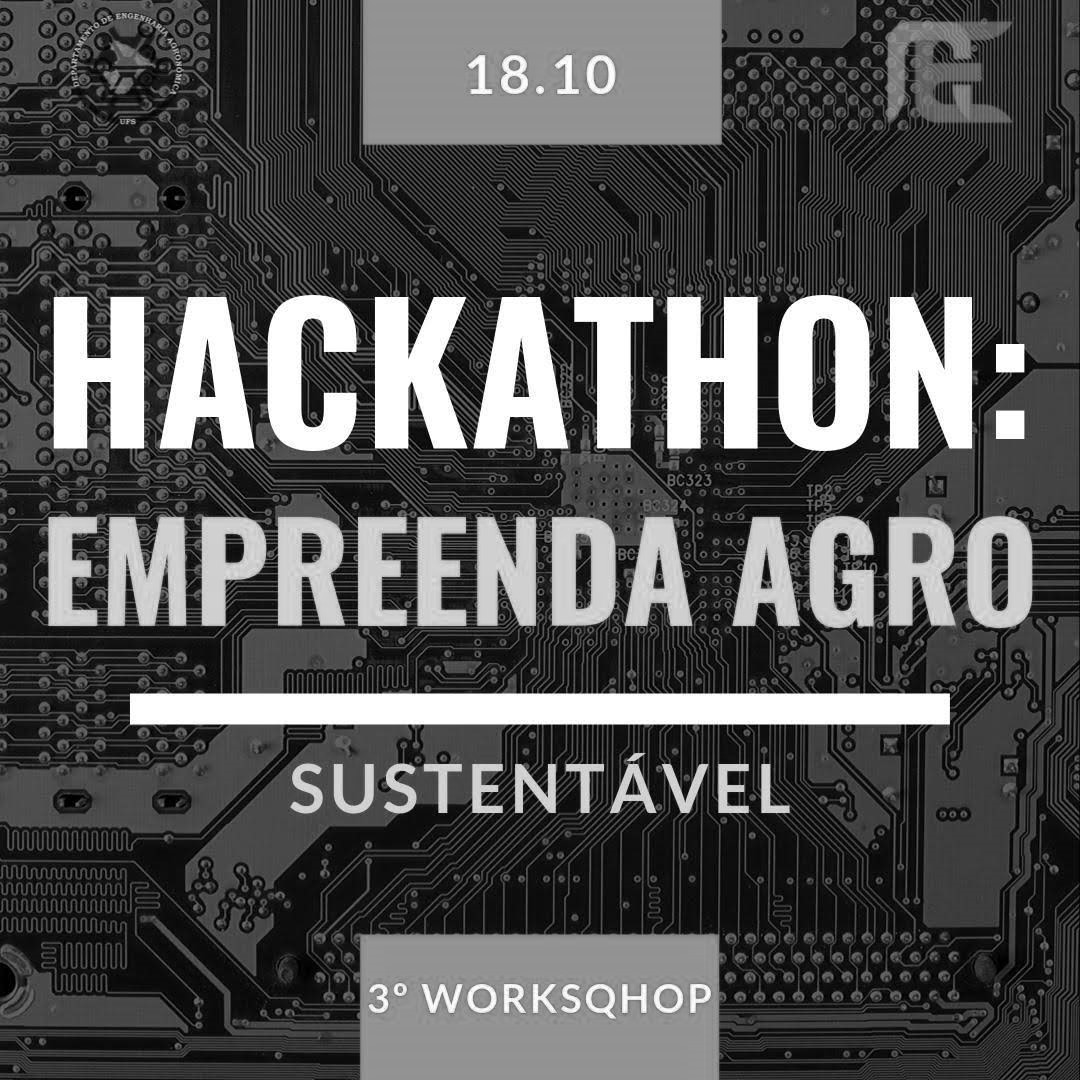
\includegraphics[scale=0.15]{Imagens/hackaton_1.jpg}}
\qquad
\subfigure[ref2][Cronograma]{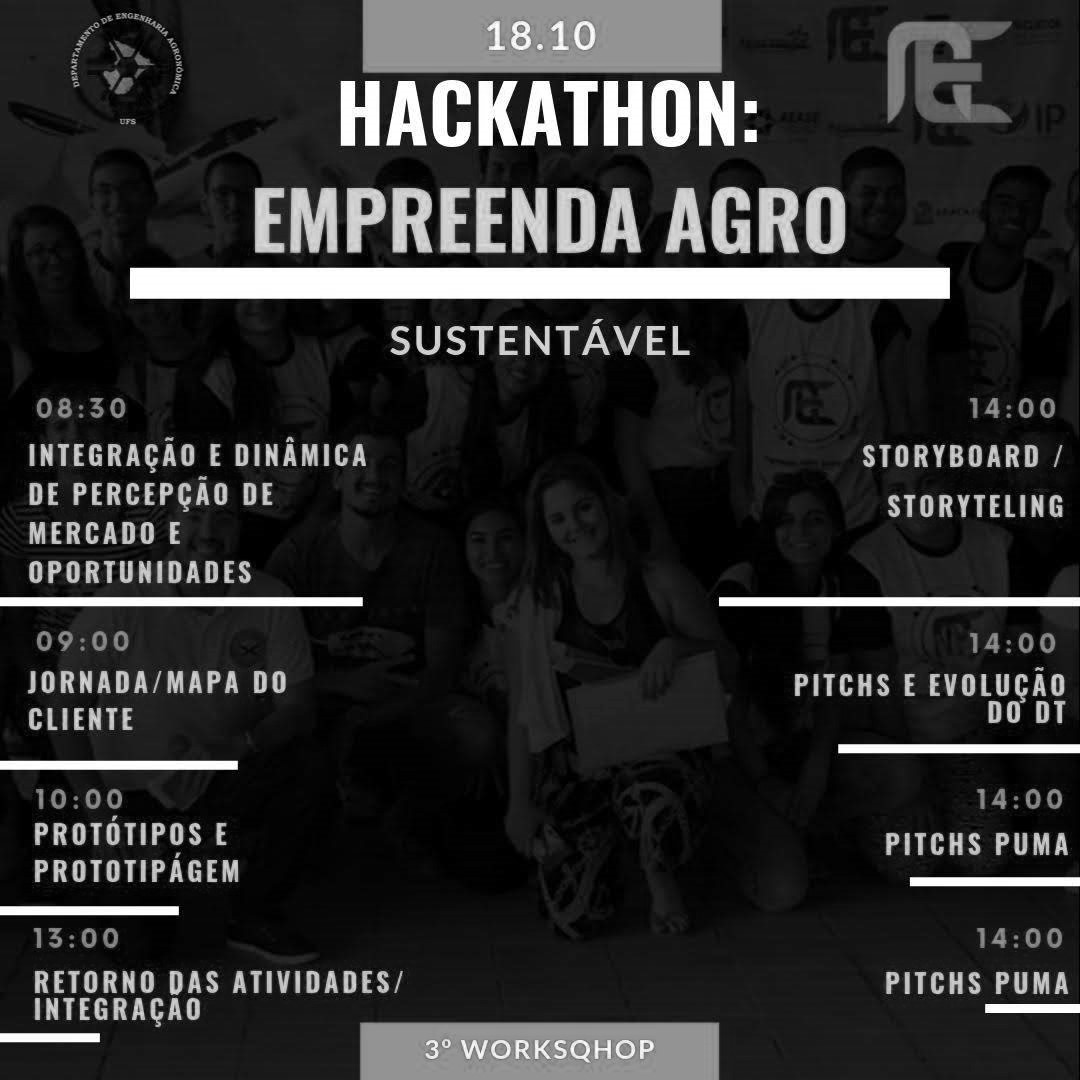
\includegraphics[scale=0.15]{Imagens/hackaton_2.jpg}}
\qquad
\fonte{O Autor}.
\label{figura_podcast}
\end{figure}




\subsection{Demoday}

O Demoday ou Dia de Demonstração dos modelos de negócios das startups foi realizado no dia 22 de novembro de 2019. Esse foi o evento em que as startups se apresentaram para investidores, que são representados por ventures capitals, aceleradoras ou investidores-anjos. Nessa oportunidade os jovens empreendedores apresentaram seus projetos em busca de investimentos. 

As 15 startups formadas pelo programa realizaram a exposição e apresentação de seus modelos de negócio e protótipos, bem como a apresentação dos pitchs de cada equipe para o público presente, além de participação em um “Talk Show” com exposição de pitchs. Dados resultantes do demoday estão descritos na Seção \ref{inovacoes}. 
O Apêndice \ref{app:workshop_demoday} (Figura \ref{figura_35}), demostra momentos ocorridos durante o encontro promovido pelo programa.



\begin{figure}[H]
\centering
\caption{\textbf{Banner divulgação Demoday}}
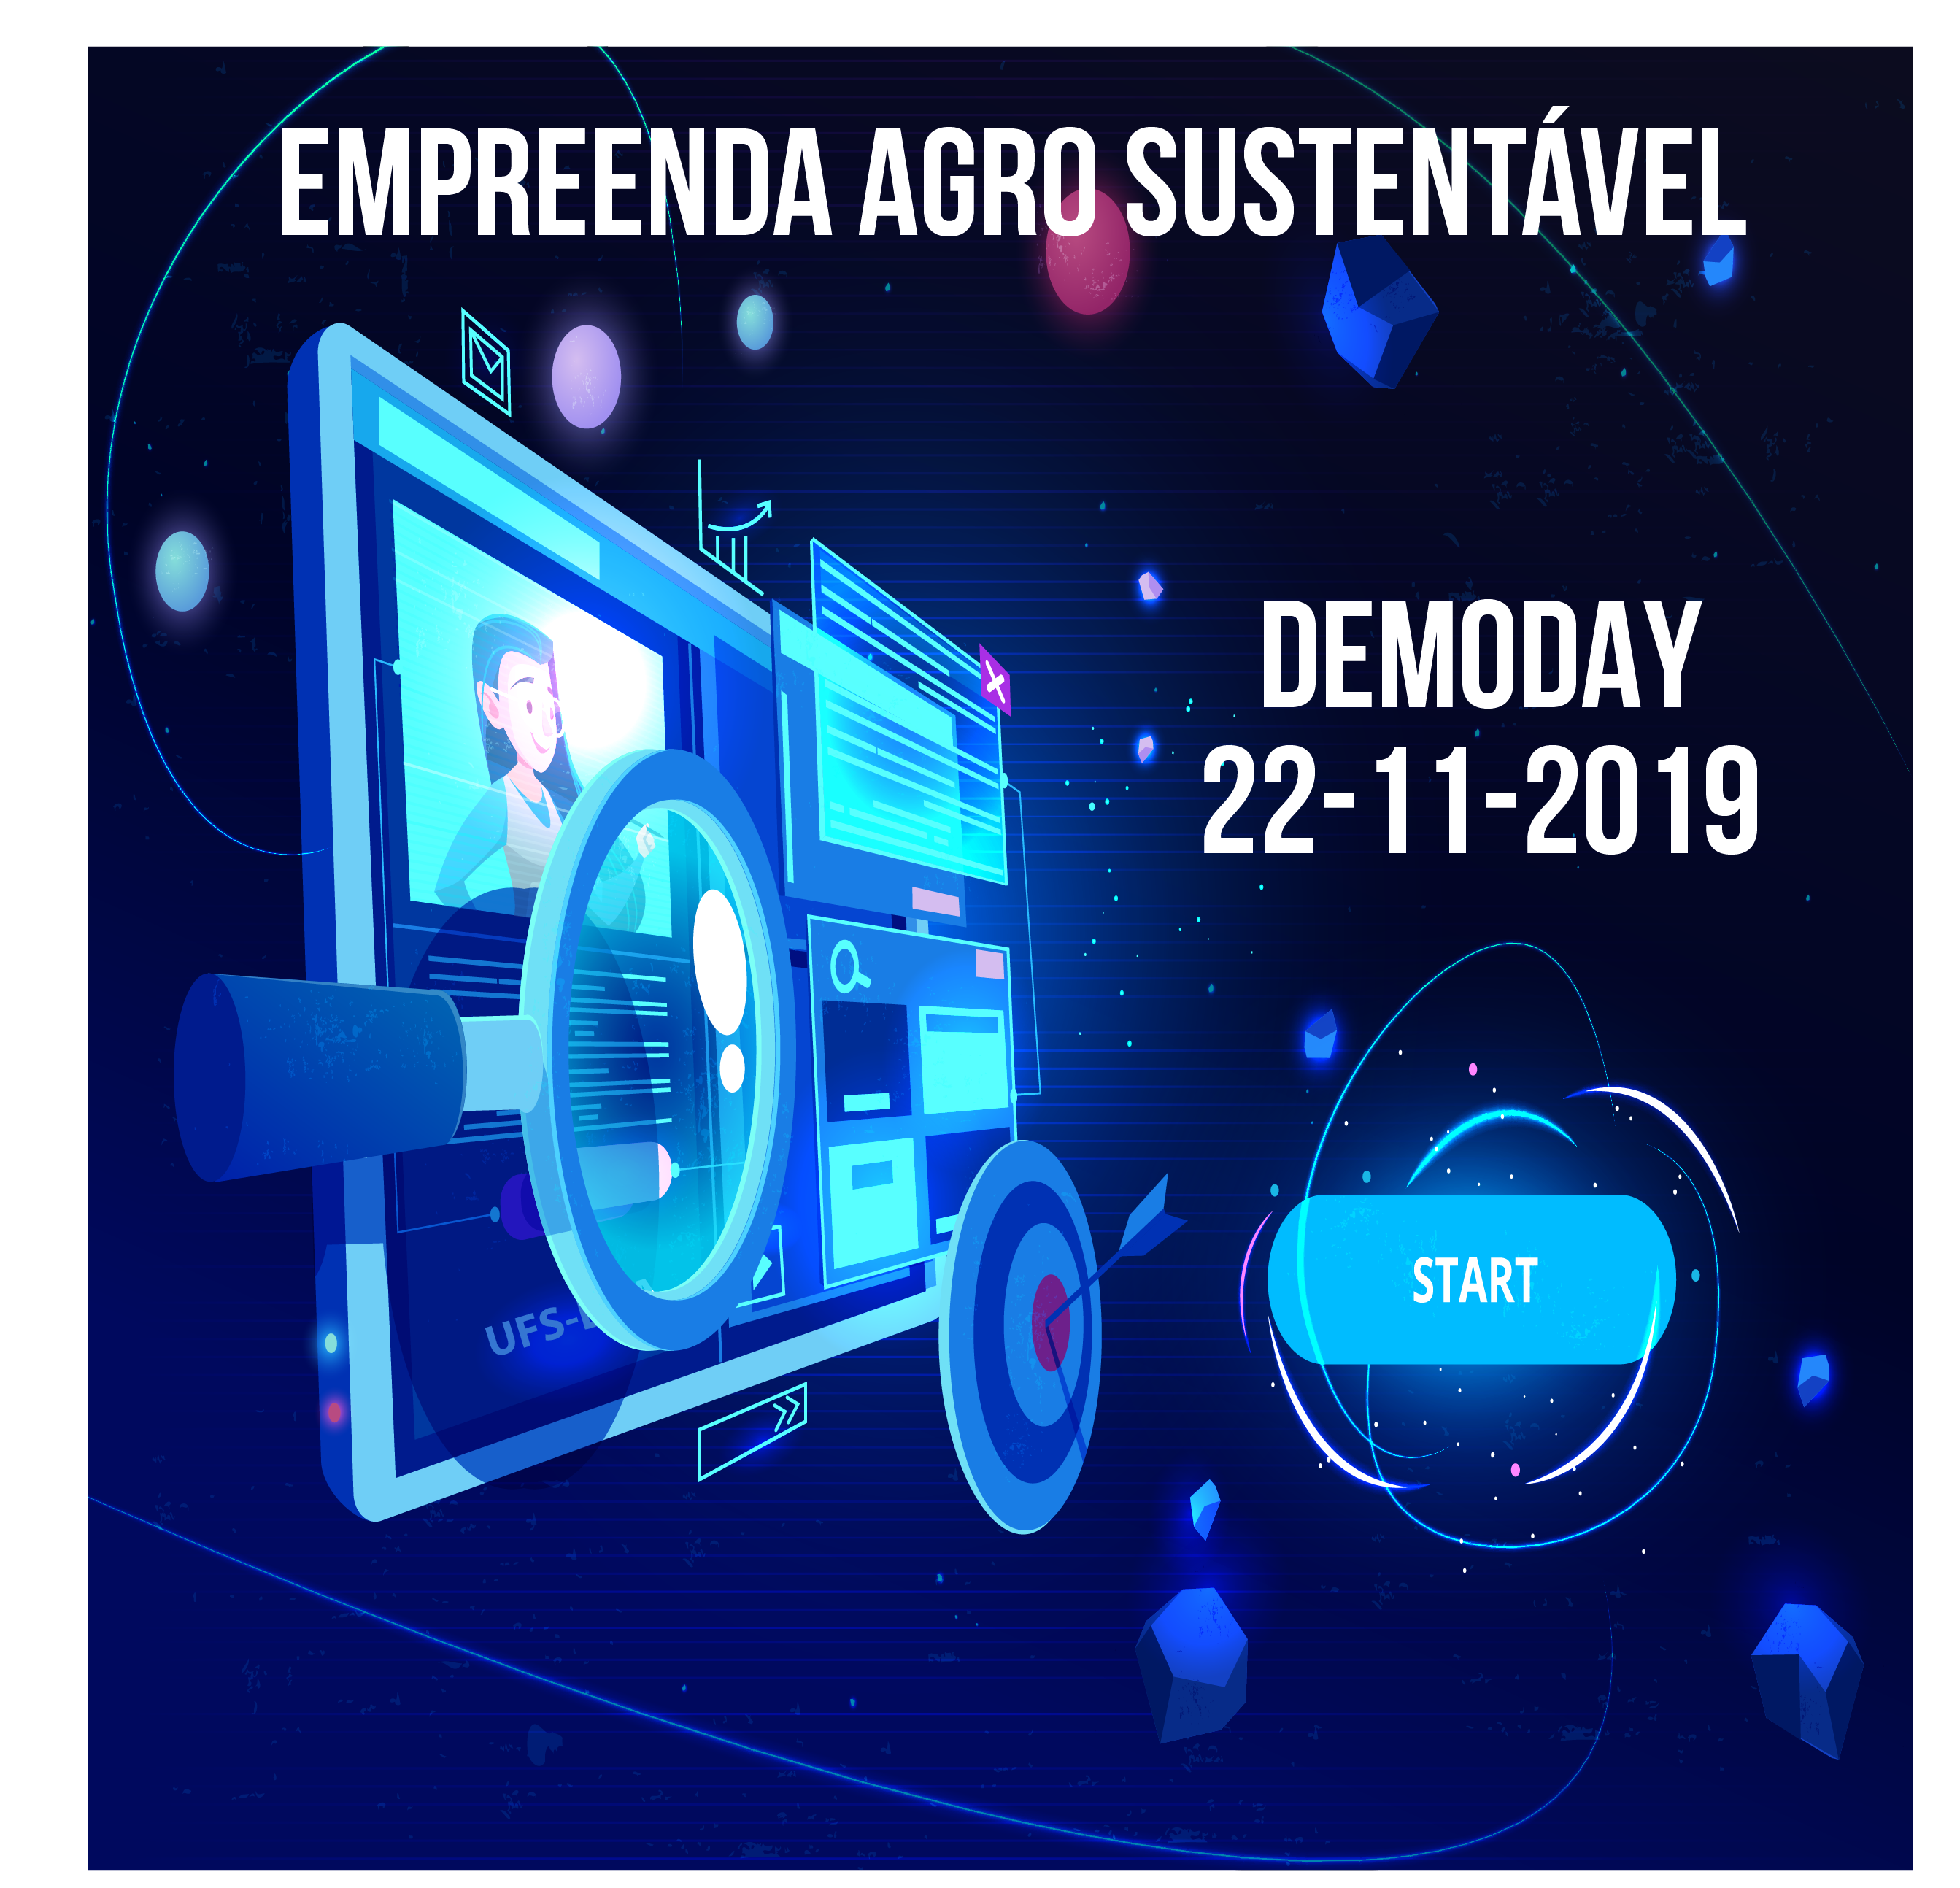
\includegraphics[scale=0.1]{Imagens/demoday_banner.png}
\fonte{O autor}
\label{fig:ods}
\end{figure}


\section{Resultado da análise do Survey utilizado}

Foi aplicado o teste de confiabilidade e agrupamento dos dados amostrais por rotação Varimax, tendo como dados de normalização o Kaiser\footnotemark[1]. 
Após análise  emergiram 3 componentes principais esperados para esta pesquisa, aglutinando as questões na ordem apresentada no apêndice \ref{chap:tabela_2} (Tabela \ref{tabela_3}).


As questões: \textbf{"Para mim sem empresa não é autônomo"} e \textbf{"Pensando em todos os possíveis recursos que minha família me fornece, eu sou completamente independente dela para decidir como alocá-los e usá-los.			
"}, foram eliminadas da pesquisa, pois foi adotado a supressão de coeficientes que apresentaram valores absolutos a baixo de 0,40, já as questões: \textbf{Assumir riscos calculados}, \textbf{Conduzir minha própria empresa ao sucesso} e \textbf{Começar minha própria empresa} (Apêndice \ref{chap:tabela_2}), apresentaram valores satisfatórios tanto para dimensão Autoeficácia quanto para dimensão intenção empreendedora, porem foi considerado o valor de coeficiente mais alto. 
A tabela \ref{tab:tabela_4}, apresenta a variância total explicada para as dimensões tratadas na pesquisa. 


\begin{table}[H]
 \centering
\caption{\textbf{Variância total explicada}}
\label{tab:tabela_4}
\hline\hline
\begin{tabular}{c c c c }
\multicolumn{1}{p{6cm}}{} & \multicolumn{3}{c}{\textbf{Fatores}}\\ 
 \multicolumn{1}{c}{\textbf{Itens}} & \multicolumn{3}{c}{\hrulefill}\\ 

 \multicolumn{1}{c}{} 
 &\multicolumn{1}{c}{\textbf{Autoeficácia}} & \multicolumn{1}{c}{\textbf{Intenção}} &\multicolumn{1}{c}{\textbf{Família}}  
\\\\ \hline 

 Somas de rotação de carregamentos ao quadrado (n)
 & 6,602 & 4,090 & 2,802 \\\\
 Variância explicada (\%)
 & 22,766 & 14,102 & 9,662\\\\
 Variância cumulativa (\%)
 & 22,766\% & 36,868\% & 46,530\% \\\hline \hline 
\end{tabular}
\fonte{O autor}.
\end{table}


Os resultados obtidos na estatística KMO apresentados nas Tabelas \ref{tabela_8} e \ref{tabela_9} respectivamente, para os dois momentos do questionário desenvolvido após o teste de rotação Varimax,  demostraram haver baixa variância entre os dados encontrados, porém o teste de esfericidade de \textit{Bartlett} demonstrou haver significância e validade para os dados já que a significância dos dados obtidos foram menores que 0,05\%, demonstrando haver ajuste dos dados à Análise Fatorial Exploratória (AFE), desta forma, os dados obtidos satisfazem o objetivo proposto na pesquisa, desde que para as análises posteriores sejam utilizados testes não paramétricos, para isto foi utilizados para análise de distribuição o método \textit{Kolmogorov-Smirnov}, da mesma forma que para os testes post-hoc foi utilizado o teste U de \textit{Mann-Whitney}.


Resultados abaixo de 0,5 indicam que a análise fatorial é insatisfatória em decorrência da correlação fraca entre as variáveis. Valores da estatística KMO acima de 0,6 confirmam a validade dos dados coletados. Na realização do teste KMO dos dados levantados, foram obtidos os resultados que seguem para os momentos da pesquisa resultados na Tabela \ref{tabela_8}.

\begin{table}[H]
\FloatBarrier
\centering
\caption{\textbf{Estatística KMO e Bartlett - Antes do programa}}
\label{tabela_8}
\begin{tabular}{ll|l}
\hline\hline
\multicolumn{2}{l|}{\multirow{2}{*}{Medida Kaiser-Meyer-Olkin de adequação de amostragem.}} &  \\
\multicolumn{2}{l|}{} & ,604 \\ \hline
\multirow{3}{*}{Teste de esfericidade de Bartlett} & Aprox. Qui-quadrado & 1041 \\
 & gl & 378 \\
 & \textit{P-value}. & ,000 \\ \hline
\end{tabular}
\fonte{O autor}
\end{table}

\begin{table}[H]
\FloatBarrier
\centering
\caption{\textbf{Estatística KMO e Bartlett - Após o programa}}
\label{tabela_9}
\begin{tabular}{ll|l}
\hline\hline
\multicolumn{2}{l|}{\multirow{2}{*}{Medida Kaiser-Meyer-Olkin de adequação de amostragem.}} &  \\
\multicolumn{2}{l|}{} & ,598 \\ \hline
\multirow{3}{*}{Teste de esfericidade de Bartlett} & Aprox. Qui-quadrado & 850 \\
 & gl & 378 \\
 & \textit{P-value} & ,000 \\ \hline
\end{tabular}
\fonte{O autor}
\end{table}

%\subsection{Interesse em conteúdos relacionados a educação empreendedora}


%Como mostra a Tabela 1, os estudantes participantes do programa se caracterizam por uma maior diferença entre
%gostaria de fazer e não tenho interesse em fazer do que os pesquisados por  \cite{lima_ser_2015} no Brasil. A única exceção ocorre para
%com empreendedores experientes. Quanto à disciplina de empresas familiares, no
%contexto da EE, ela parece reforçar a sinalização já feita pelos estudos do CFA (Andrade et al., 2006;
%Mello et al., 2011) da necessidade de conteúdo de formação em administração de micro e pequenas empresas.




\subsection{Dimensão autoeficácia empreendedora}

Considerando que os escores das perguntas relacionadas a dimensão empreendedora variam de 1, menor número, a 7, maior número na escala, foi avaliada a média de cada variável (questão),
o histograma (Figura \ref{figura_29}), foi extraído partindo da medina de cada resposta aglutinadas em fatores, onde quanto mais próximo de 7, melhor a perspectiva de mudança positiva para a amostra pesquisada que se inscreveu e participou do programa. Foi observado utilizando o Teste-t pareado com o intervalo de confiança em 95\%  que a autoeficácia para os participantes, sem levar em consideração as diferenças dos cursos, não variou significativamente (p-value 0,118), porem, observando as médias nos histogramas das respostas antes e após a participação do programa passou de 5,31 para 5,65 (Figura \ref{figura_29}) e que as respostas aumentaram a frequência para os quesitos 6 \textit{"Seguro"} e 7 \textit{"Completamente seguro"}.

A autoeficácia empreendedora é uma importante dimensão para a geração de inovação e criatividade para novos negócios e produtos escaláveis. \citeonline{gubik_student_2016} afirmam que, a auto-eficácia relacionada ao empreendedorismo e o conhecimento de processos empresariais também afetam significativamente as intenções empresariais, e que, alunos mais autoconfiantes (maior lócus de controle) têm maior autoeficácia e em consequência melhor desempenho nos negócios.


Neste sentido, as instituições de ensino superior, independente da ciência de estudo deve ser capaz de proporcionar atividades didáticas que tenham como propósito a melhoria do nível da autoeficácia dos alunos resultando numa melhora das competências empreendedoras  pós formação dos mesmos \cite{ribeiro_autoeficacia_2019}. A busca pela melhoria da dimensão da autoeficácia empreendedora ajudará a moldar o futuro dos alunos no mercado de trabalho e motivará a ter sucesso em seus futuros negócios, permitindo assim os alunos  definir e seguir o seu próprio percurso profissional com sucesso  \cite{das_examining_2018}.

\begin{figure}[H]
\centering
\caption{\textbf{
Contagem Dimensão da Autoeficácia empreendedora  por Momento da Pesquisa}}
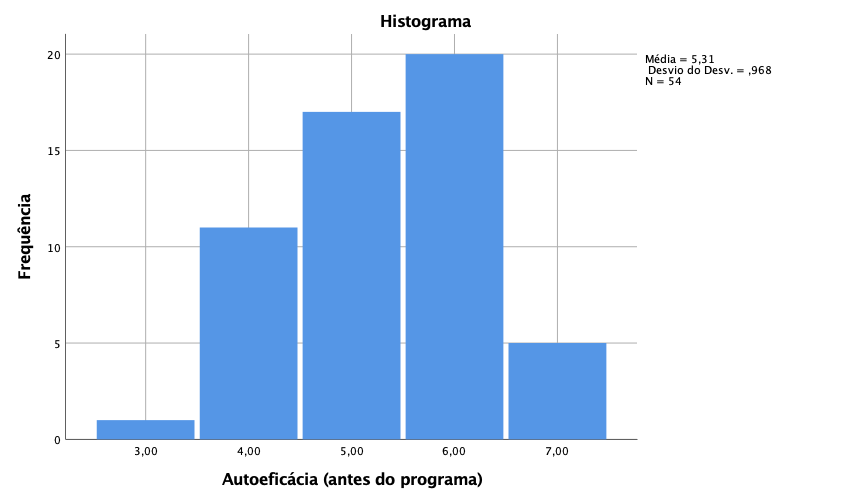
\includegraphics[scale=0.4]{Imagens/histograma_autoeficacia_antes.png}
\fonte{O autor}
\label{figura_29}
\end{figure}


Nas respostas por curso, os alunos do curso de zootécnica mostram-se mais seguros quando se compara as médias obtidas aos demais cursos participantes, saindo da média de 4,53 para 5,58. O curso apresentou um crescimento maior frequência na questão 5 \textit{um pouco seguro}, ouve um crescimento das respostas: 6 \textit{seguro} e 7 \textit{completamente seguro}, porém, os alunos que mostraram mobilidade na frequência da mediana foram os alunos matriculados no curso de engenharia agrícola, os quais saíram da questão 5 \textit{um pouco seguro} para 6 \textit{seguro}. Os alunos do curso de engenharia agronômica, passaram a se sentirem menos indecisos, mobilizando suas opiniões para as questões acima desta. O curso de engenharia de pesca não apresentou inscritos suficiente para manter uma frequência experimentável. Na figura \ref{figura_34} é possível observar a mobilidade das respostas dos alunos (aqui representado pelos quartis) após a participação no programa.


\begin{figure}[H]
\centering
\caption{\textbf{Mobilidade de respostas sobre autoeficácia por curso}}
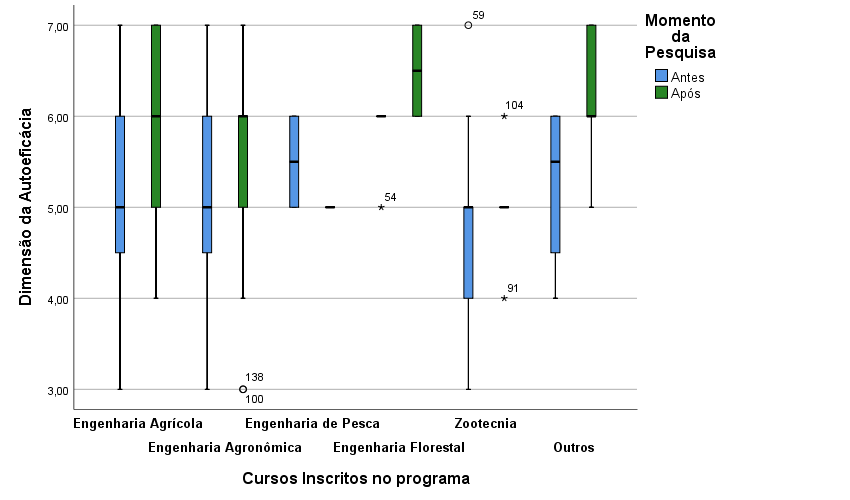
\includegraphics[scale=0.4]{Imagens/boxplot_autoeficacia.png}
\fonte{Autoria própria}
\label{figura_34}
\end{figure}


No Apêndice \ref{tab:amostras_autoeficacia} (Tabela \ref{tabela_5}), nota-se que as questões \textbf{Fazer análises financeiras"}, \textbf{"Reduzir riscos e incertezas"}, \textbf{"Assumir riscos calculados"}, \textbf{"Administrar o tempo estabelecendo metas"} e \textbf{"Conduzir minha própria empresa ao sucesso"} obtiveram valores de 0,007, 0,00, 0,024, 0,027 e 0,028 respectivamente, tais valores foram menores que o intervalo de confiança (0,05), podendo para estas questões ser rejeitado o H0 para a dimensão da autoeficácia . 


O fato de o programa Empreenda agro sustentável ter um caráter de pré-aceleração, foi pensado com o objetivo suprir uma lacuna na formação dos discentes das ciências agrárias e demais áreas da Universidade Federal de Sergipe, em relação ao desenvolvimento de um pensamento empreendedor, por meio da promoção de um ciclo de oficinas, visando a disseminação dos valores e técnicas dos gerenciamentos ágeis e a promoção do empreendedorismo capaz de aplicar tais metodologias na produção rural, pode ter influenciado na melhoria da autoeficácia para análise financeira dos negócios, a predição de riscos e possíveis mitigações, a gestão ágil do tempo e atividades relacionadas a inovação, e a promoção da disposição a assumir riscos calculados em novos empreendimentos. 

Tais resultados se aproximam com os observados por \citeonline{schafer_be_2018} sobre a mudança na autoeficácia para o empreendedorismo social, investigando as necessidades motivacionais que influenciam a intenção de potenciais empreendedores, observou que a educação para o empreendedorismo no promove a melhoria da autoeficácia empresarial, e que a desejabilidade de criar novos negócios para o âmbito social, foi determinada pela vontade dos alunos de auto realização e autonomia pessoal, após a vivência de conteúdos voltado a educação empreendedora. 

Neste sentido, levando em consideração os resultados da dimensão autoeficácia observada no estudo, não se rejeita a hipótese nula (H0) (Não há diferença entre as médias das medidas que averíguam o perfil empreendedor entre os alunos participantes do Programa de extensão Empreenda Agro Sustentável), quando observado os resultados da diferença apresentada no teste estatístico, contudo o programa empreenda agro sustentável proporciono uma mobilização positiva das respostas quando se comparado aos resultados iniciais dos participantes.



\subsection{Dimensão da participação familiar e influência de terceiros no desenvolvimento empreendedorismo}

A participação familiar se mostra pouco móvel diante das questões apresentadas (Figura \ref{figura_60}), este fator pode ser influenciar negativamente na escalabilidade do negócio planejado pelo novo empreendedor. Quando consideramos que as famílias são uma importante fonte, networking para novos negócios \cite{dieguez-soto_does_2019,raza_influence_2019,kupp_when_2019}, de financiamento em estágio inicial \cite{dieguez-soto_does_2019,edelman_impact_2016} e cuidados familiares. \citeonline{meliou_family_2020} em seu trabalho sobre família como uma bolha eudaimônica \cite{puzi_transgenerational_2020}, sugerem que o potencial transformacional dos cuidados familiares, pode influenciar positivamente para a viabilidade dos negócios e posiciona a família, em um ponto chave para o surgimento de novos negócios. 

Esta pesquisa demonstrou que a dimensão familiar não é influenciada por programas de extensão sobre educação empreendedora (Apêndice \ref{tab:amostras_familiar}, Tabela \ref{tabela_familair}).

A família costuma desempenhar importantes funções de incubação no processo de criação de novos empreendimentos, já que muitos negócios podem surgir do empreendedorismo transgeracional \cite{puzi_transgenerational_2020,meliou_family_2020}, ou da mobilização de recursos familiares, demonstrando a importância desta dimensão ser melhor estudada em futuros trabalhos, já que muitos profissionais não tem apoio familiar para desempenhar o papel de mentor para negócios, já que, as famílias são consideradas fornecedoras de “capital paciente” \cite{lumpkin_longterm_2011}. 





\begin{figure}[H]
\centering
\caption{\textbf{Contagem geral por momento da pesquisada sobre a participação familiar e influência de terceiros}}
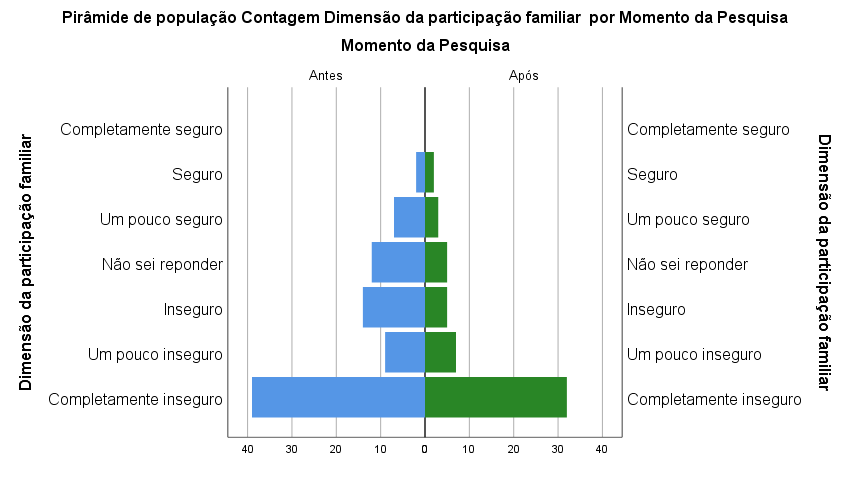
\includegraphics[scale=0.4]{Imagens/dimensao_familiar.png}
\fonte{O autor}
\label{figura_60}
\end{figure}


\subsection{Dimensão e intenção ao empreendedorismo dos estudantes}

Para impulsionar as atividades empreendedoras dos alunos, é essencial identificar os fatores que formam as intenções empreendedoras e investigar como o desenvolvimento desses fatores pode ser influenciado \cite{gubik_entrepreneurial_2019}. 

A educação afeta significativamente as intenções em relação ao empreendedorismo
A IE pode ser definida como uma intenção pessoal conduzida por ações e objetivos futuros a ser implementadas buscando o desenvolvimento de novos empreendimentos. 
A IE consiste em um fator-chave que estimula o desenvolvimento de novos negócios, bem como representa o começo do processo de criação de uma nova empresa \cite{vasconcellos-guedes_e-surveys:_2007}.

A ação empreendedora, como um rotina ocorre ao longo do tempo, começa muito antes do momento em que um indivíduo cria um negócio. Assim, como em todos os comportamentos, é necessário um processo de planejamento para atingir o estágio de Intenção ao empreendedorismo, cabendo aos centros de ensino a promoção contínua e imersão frequente aos conteúdos relacionados \cite{garcia-rodriguez_entrepreneurial_2017}. 

É possível observar na Figura \ref{figura_45} assim como os dados apresentados no Apêndice \ref{tab:amostras_intencao_empreendedora} (tabela \ref{tabela_6}), que ao participar de um programa educacional que promova atividades cadenciadas para o empreendedorismo, a intenção de empreender pode ser influenciada positivamente desta forma, a aplicação de teorias motivacionais e de processos educacionais ativos buscando o isentivo ao empreendedorismo pode ser aceita, na medida que seja tida como frequente a vivência destes conteúdos e práticas \cite{fayolle_beyond_2014}.

As questões: \textbf{"Ser empreendedor me traria grande satisfação"} e \textbf{"Uma carreira de empreendedor é atrativa para mim"} (Apêndice \ref{tab:amostras_intencao_empreendedora}, Tabela \ref{tabela_6}), apesentaram mudanças positivas no questionário analisado, tais questões relacionadas a intenção empreendedora demostra que, a melhoria da auto-eficácia, promoveu maior segurança aos participantes, influenciando diretamente na intenção empreendedora, \citeonline{adelaja_students_2018} afirmam que a EE pode fornecer aos indivíduos o conhecimento específico necessário para o desempenho das tarefas e a solução de novos problemas, fatores de suma importância ao empreendedorismo, mas para que surjam resultados satisfatórios a EE apenas não apresenta resultados, mostrando a necessidade da multidisciplinaridade dos conteúdos e apoio familiar \cite{edelman_impact_2016}, também se mostra importante a segurança financeira e interesse pessoal, dai a importância do somatório das dimensões possivelmente influenciável pelo centro promotor de ensino.


No entanto, as intenções pessoais são influenciados pelos processos de socialização e, portanto, são parcialmente determinados pelos valores culturais predominantes na sociedade \cite{schwartz_les_2006}, podendo esta, sozinha, não ser suficiente para mudar o comportamento dos alunos que vivenciam \cite{adelaja_students_2018}. 

Desta forma, a EE quando direcionada a melhoria da intenção empreendedora, deve ser tida como prática comum associada a outros conteúdos de forma pratica, e melhor vivenciada no ambiente real \cite{damanpour_phases_2006}, cabendo aos locais de ensino proporcionar o máximo destas vivências. Essa intenção, portanto, surge anteriormente  à criação de um empreendimento e pode ser considerada um dos melhores preditores de empreendedorismo bem sucedido \cite{ajzen_attitudes_1987,krueger_competing_2000,garcia-rodriguez_entrepreneurial_2017}.


O papel da educação no empreendedorismo atualmente é o tópico mais  investigado na literatura empresarial. Já que, a educação focada na promoção do empreendedorismo por meio da influencia a intensão empreendedora, os alunos adquirem o conhecimento necessário para administrar um negócio e, assim, aprendendo em consequência sobre sua aptidão empreendedora \cite{nowinski_impact_2019}, que muitas vezes eram desconhecidas por ele, em consequência melhora também a auto-eficácia \cite{egerova_does_2017} aumentando a escalabilidade para novos negócios e as chances destes serem bem-sucedidos \cite{kolstad_education_2015}.

A IE é uma função das características do nível individual e dos contextos acadêmicos e sociais, com algum grau de efeitos específicos durante a vida acadêmica, desta forma diversificar os conteúdos dos futuros profissionais é uma questão crítica que merece atenção da comunidade de ensino de engenharia \cite{gilmartin_entrepreneurial_2019}.

O estudo observou que, para as questões \textbf{"Eu já sou patrão na empresa que criei"} (Apêndice \ref{tab:amostras_intencao_empreendedora}, Tabela \ref{tabela_6}), apresentaram desempenho negativos, provável ocorrência da evasão dos alunos que participaram do primeiro questionário, ficando apenas os alunos que não são donos de negócios. 


A questão \textbf{"Se tivesse oportunidade e os recursos eu me tornaria um empreendedor"} (Apêndice \ref{tab:amostras_intencao_empreendedora}), apresentou diferença positivamente significativa, é sabido que a IE antecede o passo de criação do negócio, embora nem sempre é o principal componente para surgimento de novos negócios, restrições financeiras e falta de informação e a capacidade de acumular capital específico (que é aprendido com parentes que eram empreendedores), podem ser fatores que interfiram na abertura de novos negócios mesmo que esteja presente a Intenção de empreender \cite{auguste_what_2016}.



\begin{figure}[H]
\centering
\caption{\textbf{Contagem geral por momento da pesquisada sobre a dimensão Intenção Empreendedora}}
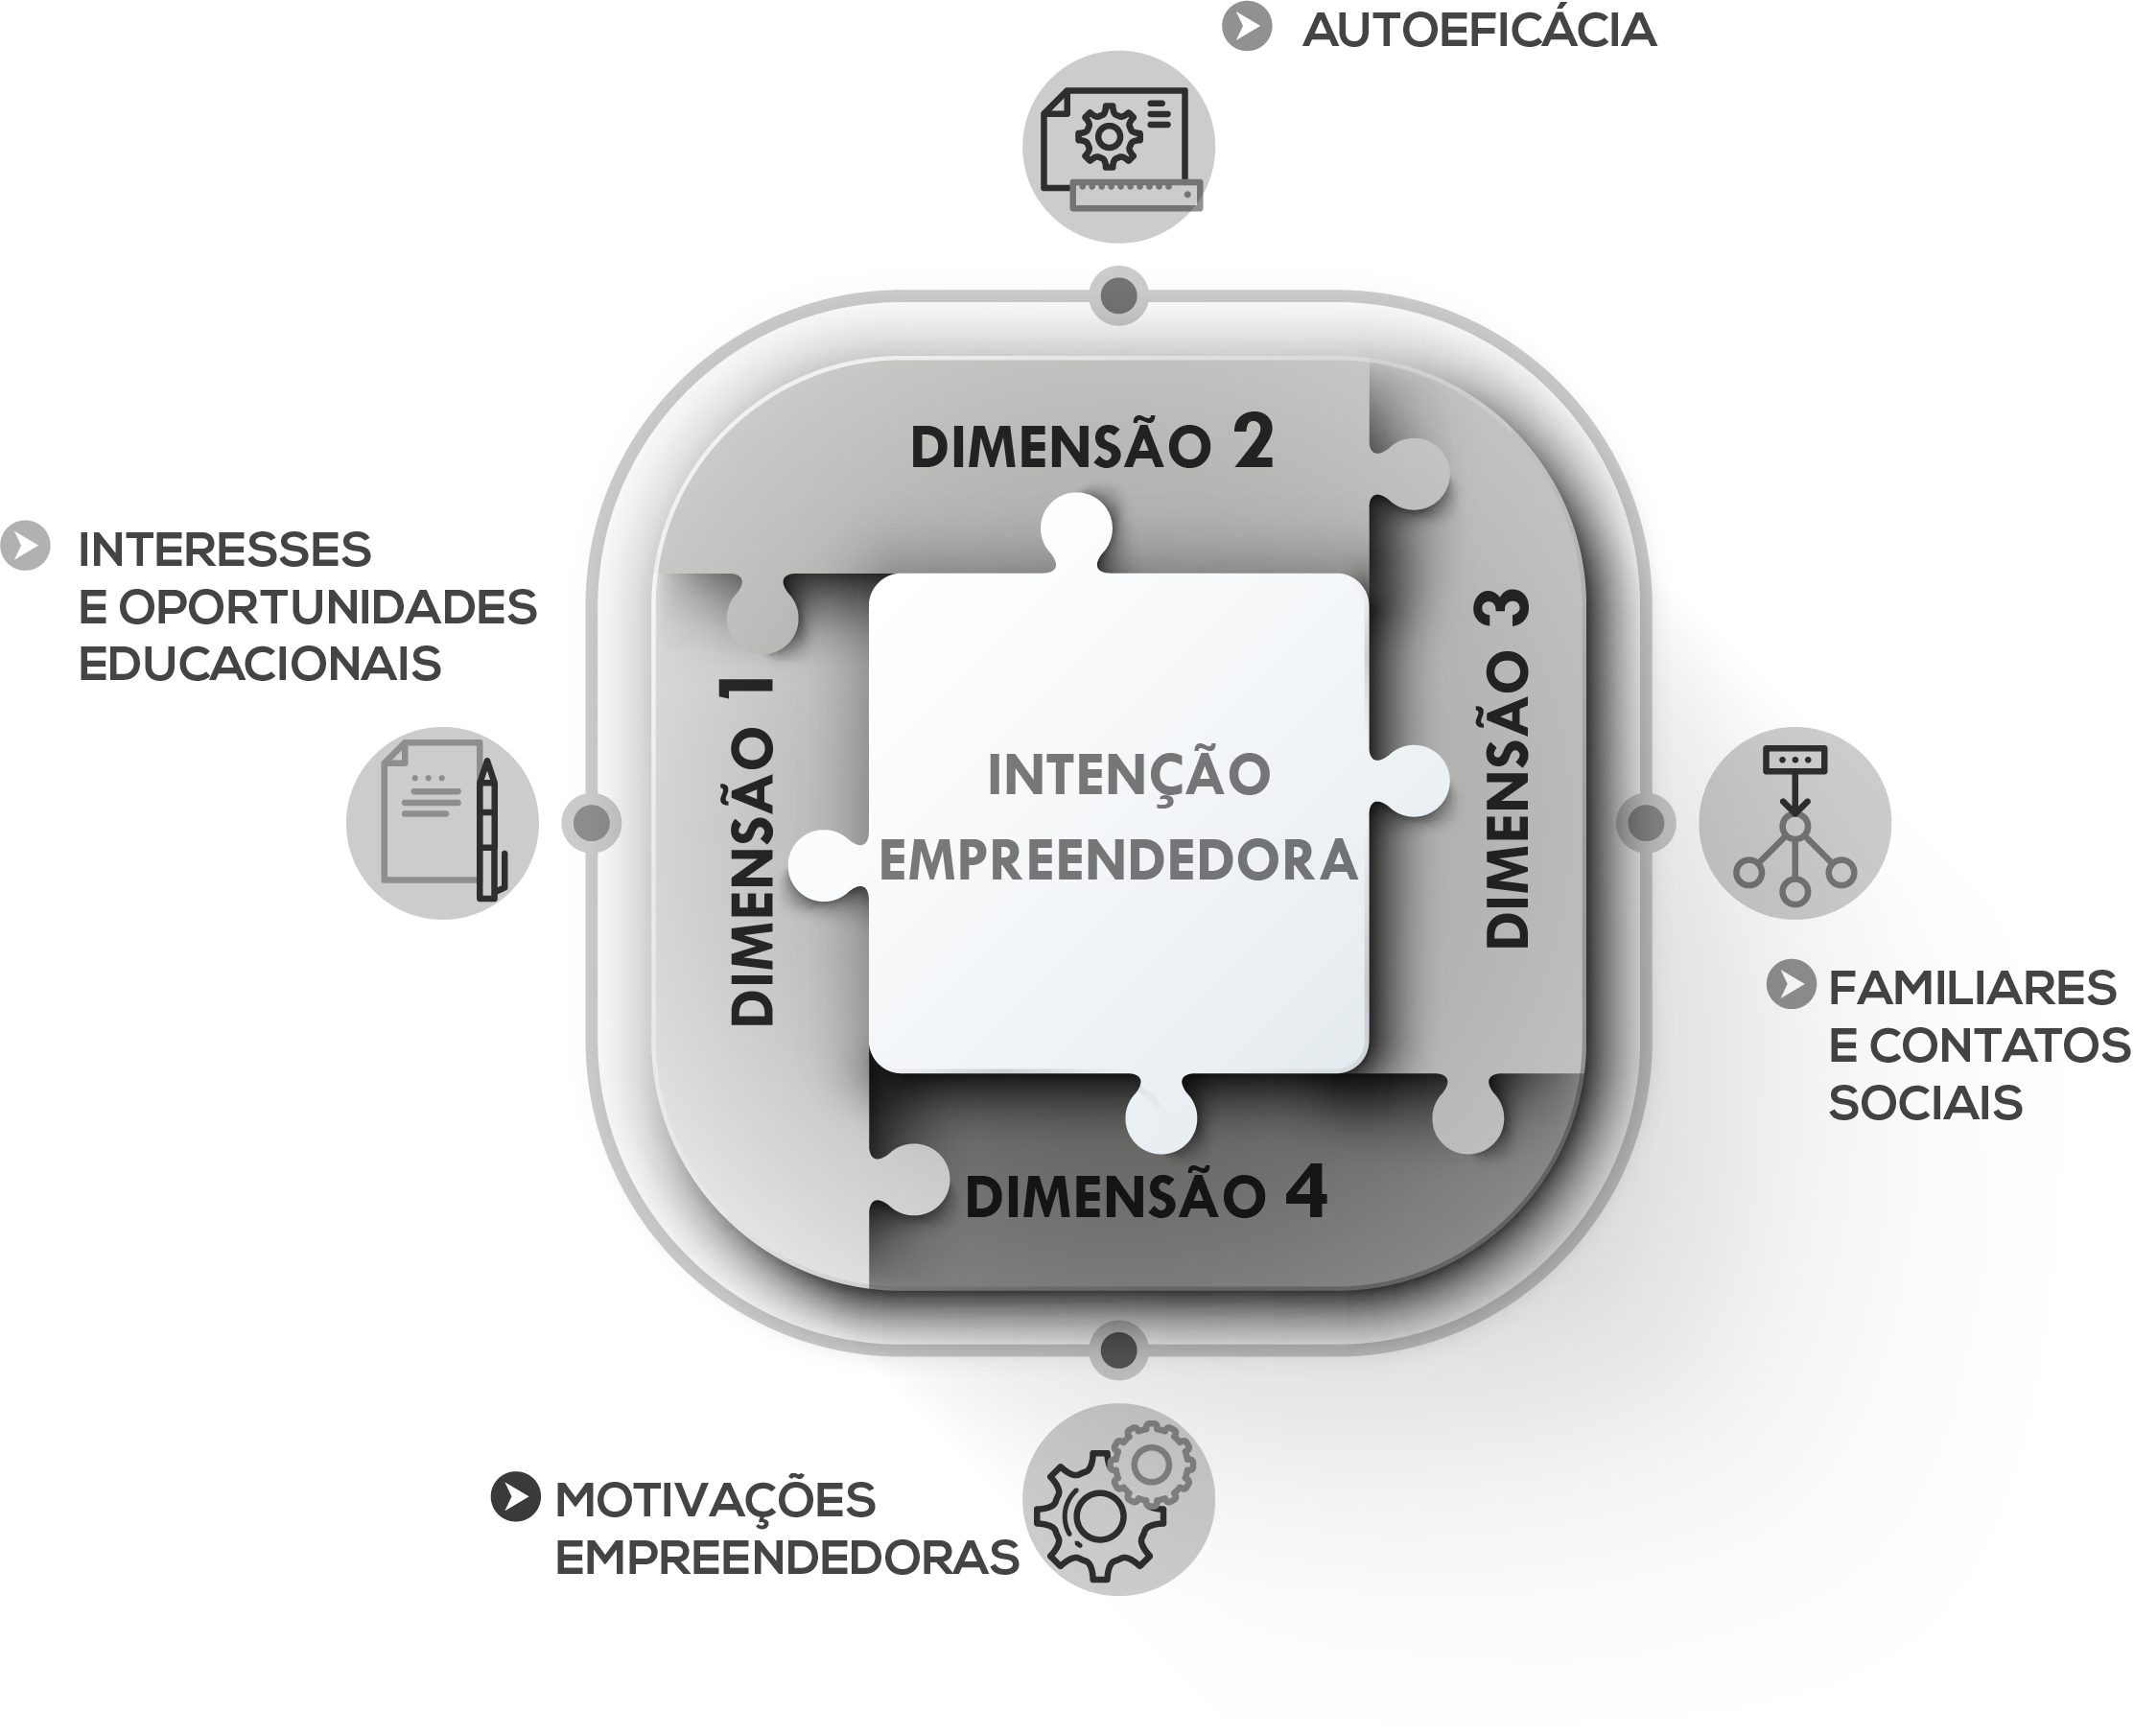
\includegraphics[scale=0.4]{Imagens/intencao_empreendedora.png}
\fonte{O autor}
\label{figura_45}
\end{figure}




\section{Inovações desenvolvidas: Marcas e Produtos}
\label{inovacoes}

O programa foi concluído  com a participação de 15 equipes (Aqua plant, Be Soluções, La Flora Pet, Agrion, Grão Nordestino, MAMP, AGROPEC, Horta House, Ranagro, Agro View, Itecagro, Tecno Coco, BAgrotec, Impacto Pescados, Uneagro), resultando ao final com 16 marcas, 15 para os grupos e a marca própria do programa, como mostrado  \ref{figura_12}.

%\begin{multicols}{3}
%\centering
%    \begin{itemize}
%\item {(a) Aqua plant;}
%\item {(b) Agrion;}
%\item {(c)AGROPEC;}
%\item {(d) Agro View;}
%\item {(e) BAgrotec;}
%\item {(f) Be Soluções;}
%\item {(g) Grão Nordestino;}
%\item {(h) Horta House;}
%\item {(i) Itecagro;}
%\item {(j) Impacto Pescados;}
%\item {(l) La Flora Pet;}
%\item {(m) MAMP;}
%\item {(n) Ranagro;}
%\item {(o) tecno Coco;}
%\item {(p) Uneagro;}
%\end{itemize}
%\end{multicols}



\begin{figure}[H]
\centering
\caption{\textbf{Portfólio das marcas desenvolvidas durante o programa}}
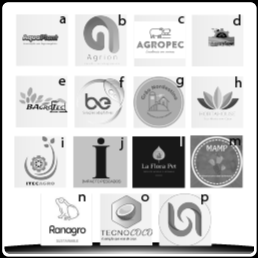
\includegraphics[scale=1]{Imagens/portfolio.png}
\fonte{O autor}
\label{figura_12}
\end{figure}


\subsection{Aqua plant}



A Startup visa justamente acabar com as incertezas que  afligem o agricultor quanto á sua produção, visto que nosso produto é um sistema de aquaponia fechado, com recirculação de água, ao qual no final do processo o produtor terá garantido proteína e hortaliças de qualidade. 

Venderemos nosso produto, que irá integrado em pacotes de assistência técnica, tanto diretamente ao produtor como também em contratos com municípios. Nossa equipe é formada por 3 estudantes de Engenharia Agronômica e 2 Engenheiros de pesca, e por meio desse ciclo a AquaPlant irá fazer produzir no Sertão. A Figura \ref{figura_13} apresenta a marca da startup. Os produtos podem ser visto no Apêndice \ref{app:workshop_demoday} página 121. 


\begin{figure}[H]
\centering
\caption{\textbf{Marca Aquaplant}}
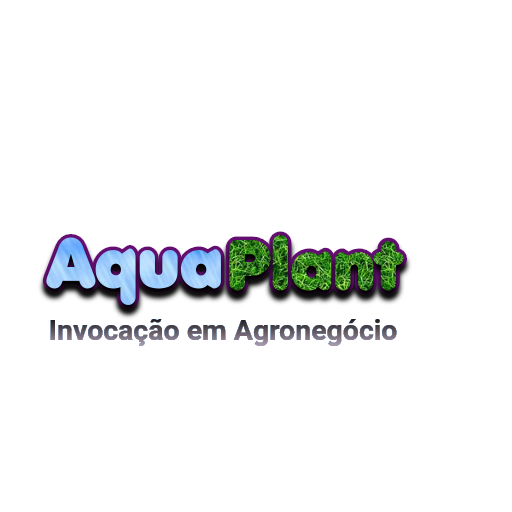
\includegraphics[scale=0.5]{Imagens/aquaplant.png}
\fonte{\cite{ufs_empreenda_2019}}
\label{figura_13}
\end{figure}


\subsection{Agrion}

Aplicativo desenvolvido por sistemas digitais afim de conectar diretamente os aplicativos desenvolvido para sistemas produtores aos mercados varejistas no processo de compra e venda de produtos agrícolas onde a lucratividade é prevista por meio da cobrança de taxação em cima do montante total de vendas diferenciando valores de venda em atacado e varejo, e porcentagem por tipo de produto.

O grande número de produtores agrícolas  do mercado sergipano com relativo que  em sua grande maioria são oriundos da agricultura familiar e ao mesmo tempo um contingente potencial de consumidores em uma curta distância. Isso baseado na  participação das cooperativas desses produtos que de acordo 
com federação tem mais de 75 cooperados e que, as mesmas têm demostrado ter capacidade de suprir o aumento da demanda. A marca pode ser vista na figura \ref{figura_14}, já os produtos podem ser visto no Apêndice \ref{app:workshop_demoday} página 118.


\begin{figure}[H]
\centering
\caption{\textbf{Marca Agrion}}

\includegraphics[scale=0.07]{Imagens/agrion.png}
\fonte{\cite{ufs_empreenda_2019}}
\label{figura_14}
\end{figure}

\subsection{BAgrotec}

Com o App TecAgro iremos conectar o produtor ao profissional, solucionando problemas no campo e consequentemente, gerando mercado de trabalho para os profissionais. Além do app o site da BAgroTec irá auxiliar no cadastramento de produtores que tiverem dificuldades com a plataforma mobile.  

O aplicativo irá valorizar o profissional gerando currículo dentro da plataforma  produtor terá acesso e retorno Imediato do profissional. Irá e fornecerá dados que irá auxiliar o profissional na tomada de decisão no campo

Muito mais que ofertar serviços de assistência técnica estamos ofertando qualidade na produção e mudaremos o atual cenário da desvalorização do profissional das agrárias. A marca pode ser vista na Figura \ref{figura_15}, já os produtos podem ser visto no Apêndice \ref{app:workshop_demoday} página 119.

\begin{figure}[H]
\centering
\caption{\textbf{Marca BAgrotec}}

\includegraphics[scale=0.9]{Imagens/bagrotec.png}
\fonte{\cite{ufs_empreenda_2019}}
\label{figura_15}
\end{figure}


\subsection{AGROPEC}


A proposta da Startup, é aproximar a indústria frigorifica dos  produtores rurais, gerindo os rebanhos, administrando um 
confinamento coletivo, comercializando animais terminados para os frigoríficos e vendendo matrizes e reprodutores em plataformas de vendas online. Iniciaremos o trabalho com 10 fazendas e um rebanho geral de 1000 matrizes, sendo planejado triplicar o rebanho atendido até o final do sétimo ano e faturar anualmente pouco mais de dois milhões de reais.

O modelo de negócio está baseado na produção de carne de  cordeiro com eficiência zootécnica e na gestão financeira, além 
da bonificação dos resultados, compra e venda de produtos  agrícolas onde a lucratividade é prevista por meio da cobrança de taxação em cima do montante total de vendas diferenciando valores de venda em atacado e varejo, e porcentagem por tipo de produto. A marca pode ser vista na Figura \ref{figura_18}, já os produtos podem ser visto no Apêndice \ref{app:workshop_demoday} página 120.


\begin{figure}[H]
\centering
\caption{\textbf{Marca AGROPEC}}
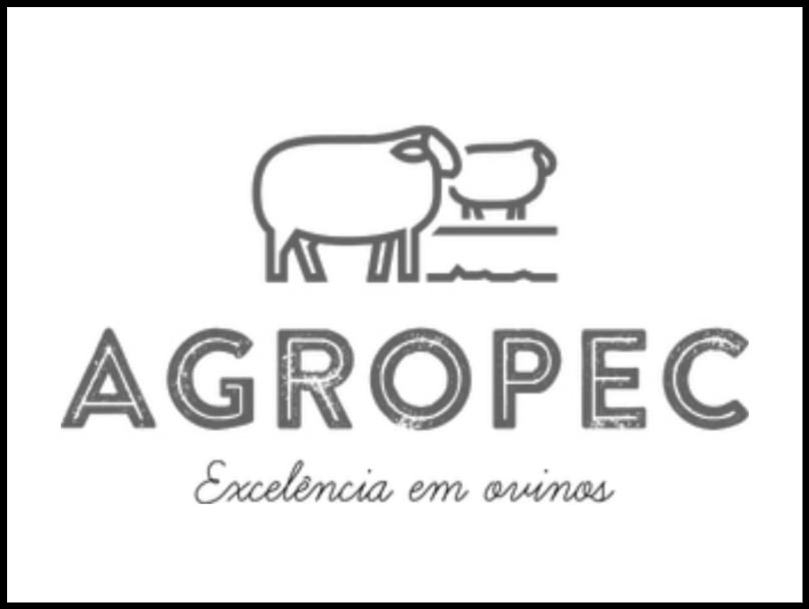
\includegraphics[scale=0.2]{Imagens/agropec.jpg}
\fonte{\cite{ufs_empreenda_2019}}
\label{figura_18}
\end{figure}

\subsection{Agro View}


Os Agroview, para terem um monitoramento mais intensivo da  produção terão que fazer um contrato mensal com a 
sua lavoura, afim de ser mais assertivo na identificação e tomada de decisão de aplicar os produtos  na hora certa, controlando antes que as pragas possam causar danos severos a lavoura, e assim  evitando uso desnecessário dos agrotóxicos. O controle quando necessário, será realizado com o uso de um drone, para dar mais agilidade ao processo e eficiência principalmente em local de difícil acesso, onde pessoas e até máquinas conseguiriam chegar, caso  de áreas muito declivosas. Essa empresa é composta por três engenheiros Agrônomos e um Engenheiro Agrícola, preparados para fazer controle biológico, seguindo  essa  visão sustentável que  já é uma tendência global. Temos um mercado gigante e promissor a ser  conquistado não só no Brasil, mas também no mundo inteiro.

Onde a startup irá disponibilizar todos os nossos serviços e  osso modelo de negócio é baseado em assinaturas mensais assistência técnica ao produtor rural. E também contratos emergenciais. Ademais, nosso cliente pode entrar em contando por meio de telefone celular e redes sociais. A marca pode ser vista na Figura \ref{figura_19}, já os produtos podem ser visto no Apêndice \ref{app:workshop_demoday} página 121.


\begin{figure}[!htb]
\centering
\caption{\textbf{Marca Agro View}}

\includegraphics[scale=0.13]{Imagens/agroview.jpg}
\fonte{\cite{ufs_empreenda_2019}}
\label{figura_19}
\end{figure}


\subsection{Be Soluções}

No atual cenário global, há cada vez uma maior demanda por métodos produtivos mais sustentáveis, especialmente quando relacionados a recursos hídricos. De acordo com a Agência Nacional de Águas (ANA), o Brasil está entre os dez países com a maior área irrigada, com cerca de 6,95 milhões de hectares (Mha), que produzem alimentos utilizando diferentes técnicas de irrigação. Segundo o Sistema Nacional de Informações sobre o Saneamento (SNIS), calcula-se que no Brasil o consumo médio de água é de 10,4 trilhões de litros ao ano, onde deste total, pouco mais de 7 trilhões são destinados à agricultura, e que deste 7 trilhões destinado a este setor, aproximadamente 3 trilhões são desperdiçados devido ao mau uso.

Para reduzir essa problemática propomos a utilização de um sistema. Um pacote tecnológico com sensores instalados em campo, que coletam dados importantes como: umidade, temperatura e condutividade elétrica, tudo em tempo real, que serão transmitidos sem fio para uma central eletrônica para um controle preciso do sistema
de irrigação, permitindo o uso mais eficiente e sustentável dos recursos hídricos.

Para reduzir essa problemática propomos a utilização de um sistema. Um pacote tecnológico com sensores instalados em campo, que coletam dados importantes como: umidade, temperatura e condutividade elétrica, tudo em tempo real, que serão transmitidos sem fio para uma central eletrônica para um controle preciso do sistema de irrigação, permitindo o uso mais eficiente e sustentável dos recursos hídricos.

Diferente dos sistemas atuais que possuem um alto custo e que não apresentam tantos recursos de forma unificada em um só equipamento, buscamos desenvolver um produto que proporcione uma alta precisão ao utilizar um sistema de dados coletados em tempo real, obtidos no local especifico da cultura. Esse equipamento é adaptativo as diferentes culturas e tipos de solo. Através de uma simples configuração na central eletrônica, por meio de uma de tela \textbf{touch} e interface intuitiva, é possível realizar uma irrigação precisa com somente a quantidade de água que a cultura selecionada necessite. A marca pode ser vista na Figura \ref{figura_20}, já os produtos podem ser visto no Apêndice \ref{app:workshop_demoday} página 122.

\begin{figure}[H]
\centering
\caption{\textbf{Marca Be Soluções}}
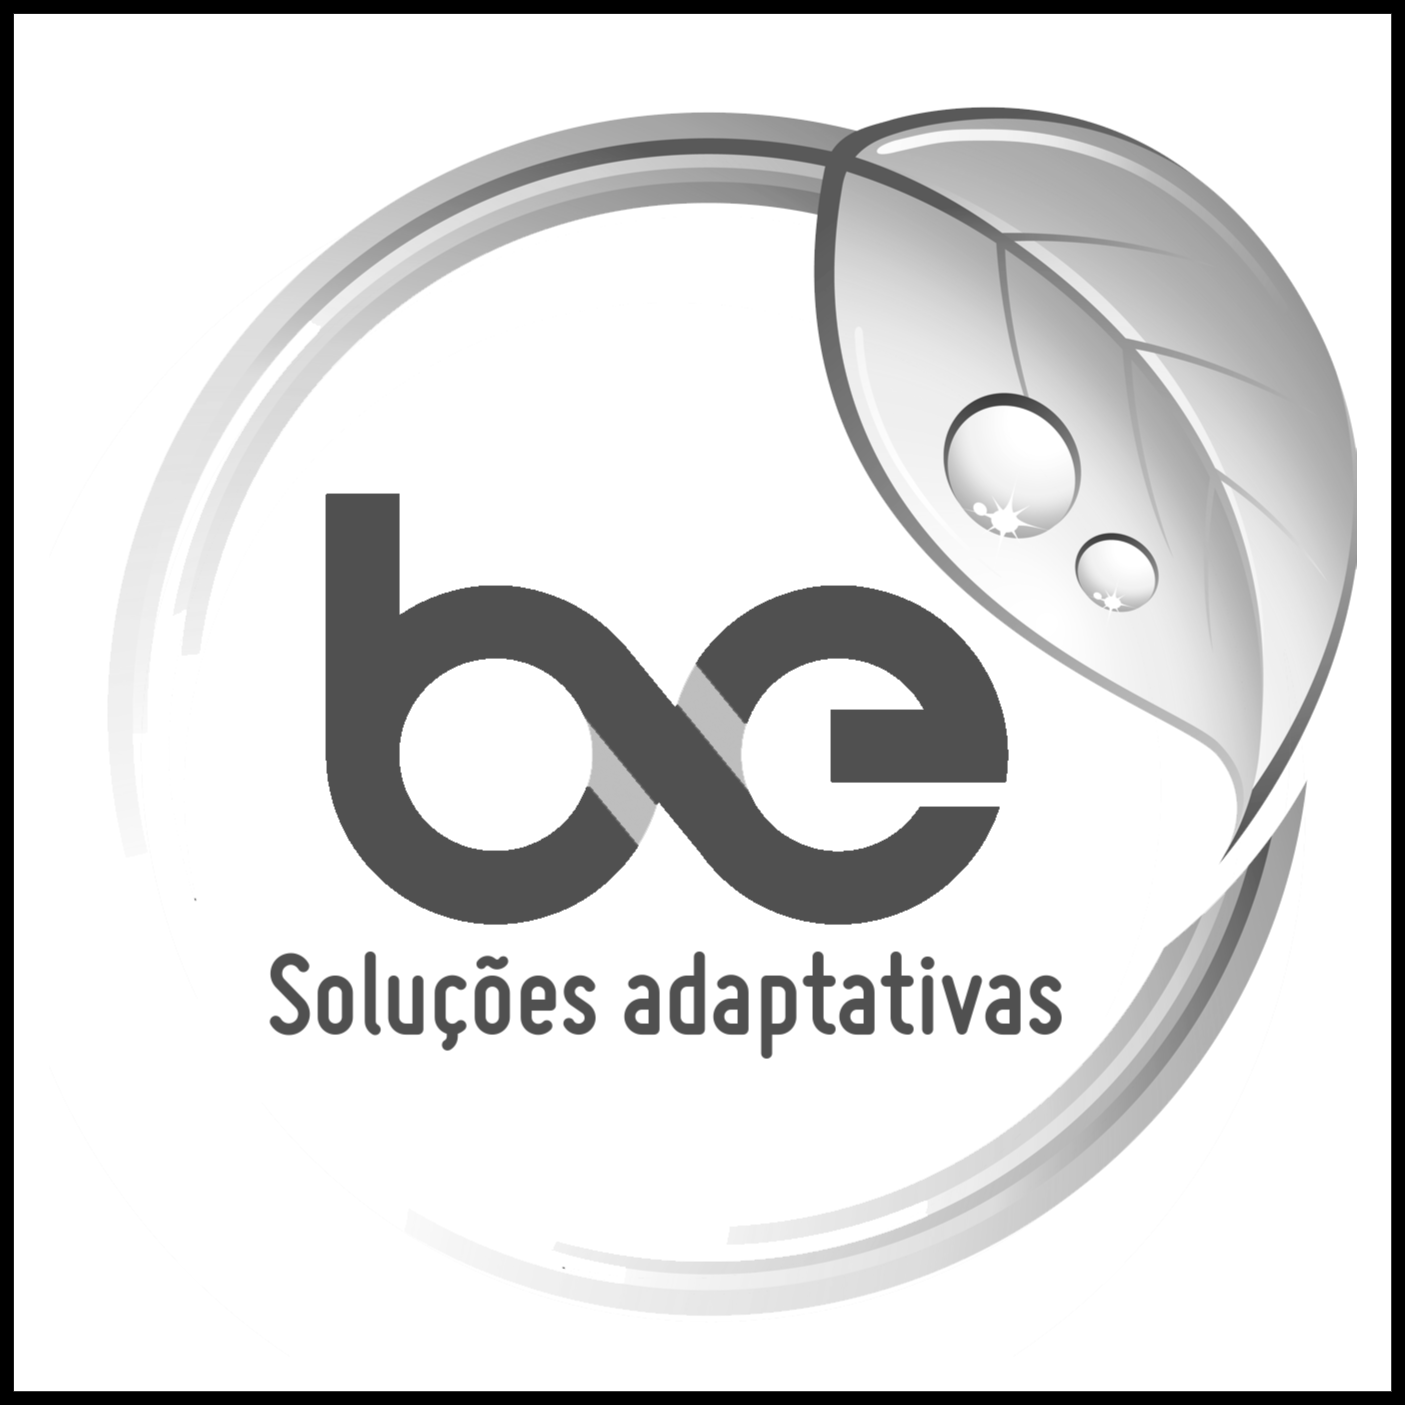
\includegraphics[scale=0.11]{Imagens/besolucoes.png}
\fonte{\cite{ufs_empreenda_2019}}
\label{figura_20}
\end{figure}




\subsection{Grão Nordestino}

Conhecendo a realidade do pequeno e médio produtor que por falta de uma unidade armazenadora perdem boa parte da sua colheita ou são obrigados a vender com o menor preço para que não venha a perder seu produto, nós da grão Nordestino trazemos o que vem a ser a solução para esse problema, projetando e instalando silos de baixo custo e sustentáveis, agregando valor ao seu produto e combatendo o desperdício de alimentos mal armazenados.

O produtor terá acesso e retorno Imediato do profissional, irá valorizar o profissional gerando currículo dentro da plataforma e fornecerá dados que irá auxiliar o profissional na tomada de decisão no campo. A marca pode ser vista na Figura \ref{figura_21}, já os produtos podem ser visto no Apêndice \ref{app:workshop_demoday} página 123.


\begin{figure}[H]
\centering
\caption{\textbf{Marca Grão Nordestino}}
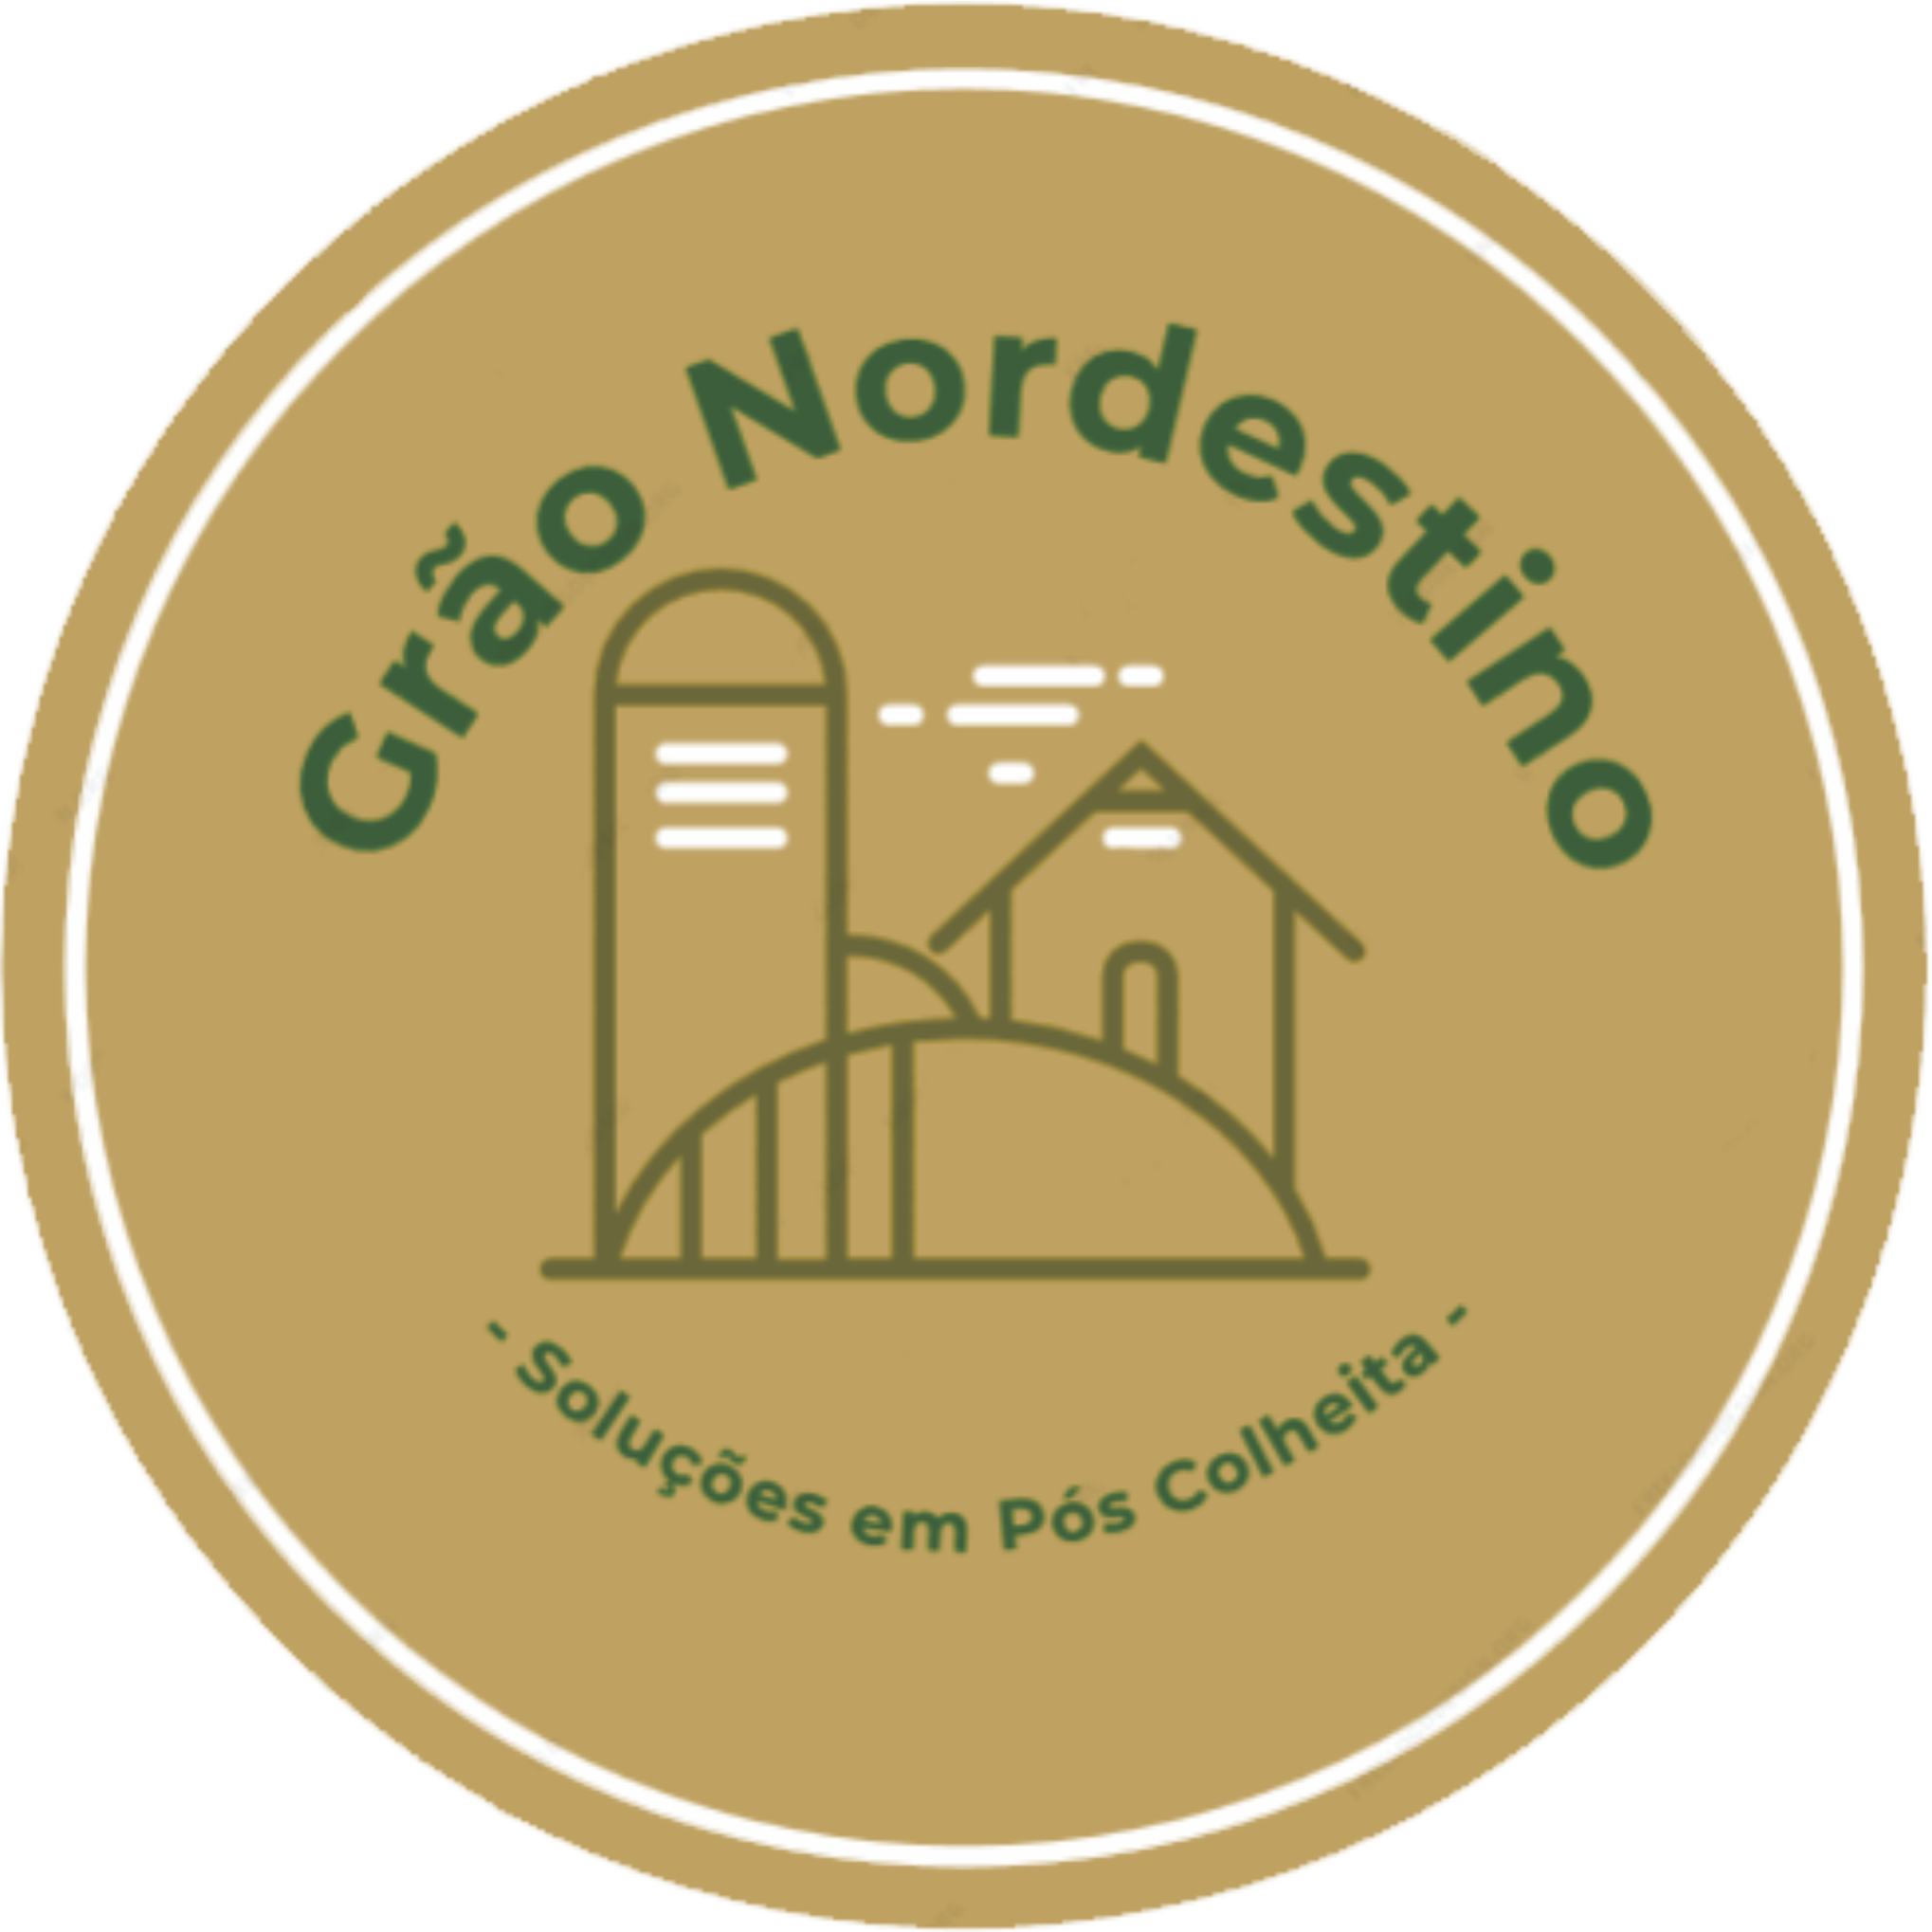
\includegraphics[scale=0.07]{Imagens/graonordestino.png}
\fonte{\cite{ufs_empreenda_2019}}
\label{figura_21}
\end{figure}



\subsection{Horta House}


O número de empresas especializadas em consultoria para hortas urbanas ainda é insuficiente para atender essa demanda que continua a crescer, tentando solucionar esse problema muitas pessoas recorrem a ferramentas de busca na internet e acabam tomando como base instruções de pessoas que muitas vezes não possuem uma qualificação para recomendações técnicas, o que em alguns casos acaba fazendo com que as plantas cultivadas entrem em um processo inverso ao desejado, ou seja morrem,

Visando solucionar esses problemas nossa empresa pretende fornecer consultoria técnica de qualidade, tendo em vista que nossa equipe é formada por três engenheiros agrônomos. Junto a nossa
consultoria pretendemos ofertar a construção de hortas planejadas de forma a que as mesmas se adéquem as necessidades do cliente, sendo incluído nesse planejamento o fornecimento de substrato, soluções nutritivas e adubos orgânicos, além das mudas. A marca pode ser vista na Figura \ref{figura_25}, já os produtos podem ser visto no Apêndice \ref{app:workshop_demoday} página 124.


\begin{figure}[H]
\centering
\caption{\textbf{Marca Horta House}}

\includegraphics[scale=0.08]{Imagens/hortahouse.png}
\fonte{\cite{ufs_empreenda_2019}}
\label{figura_25}
\end{figure}



\subsection{ItecAgro}

Plataforma de interação direta com uma equipe multidisciplinar voltada
para o agro, que se utiliza de sistemas digitais para dinamizar seu negócio de forma: Inovadora, Empreendedora e Sustentável; Propor um canal facilitador, através de sistemas digitais para dinamizar o negócio da agricultura de forma inovadora, empreendedora, e sustentável.
Tem a visão de Ser uma startup de referência desenvolvendo soluções através da assistência técnica de qualidade gerando valor ao produtor e promovendo responsabilidade socioambiental, e trabalho com excelência.
Seguindo os valores de: Inovação, Humanização, Sustentabilidade, Ética, Transparência, Profissionalismo, Confiabilidade e Tecnologia. A marca pode ser vista na Figura \ref{figura_46}, já os produtos podem ser visto no Apêndice \ref{app:workshop_demoday} página 125.

\begin{figure}[!htb]
\centering
\caption{\textbf{Marca Itec Agro}}

\includegraphics[scale=0.05]{Imagens/itecagro.png}
\fonte{\cite{ufs_empreenda_2019}}
\label{figura_46}
\end{figure}
\newpage


\subsection{Impacto Pescados}

Empresa especializada na criação de camarão do tipo \textit{Litopenaeus vannamei} com a utilização de bomba movida a óleo diesel para sucção da água do mar viabilizando as trocas de água com uma maior frequência tornando o menor tempo de cultura lançando no mercado um produto de qualidade com um menor período de cultivo. Em outras palavras baixamos o tempo de cultivo para 30 dias. A despesca do camarão de 10 gramas. O cultivo pesquisado num criador comum, foram necessários 70 dias para mesma gramatura. Custa-se, dessa forma, 5,00 R\$kg do camarão cinza. Podendo, assim, vender o produto a 15,0 0R\$ no mínimo. Segundo a Embrapa a pesca mundial não supre a demanda por pescados, ou seja, há um problema no equilíbrio entre a oferta e a demanda. Além disso, existe o fato do preço elevado para o camarão. Sendo assim, soluciona-se esta problemática com criação de camarão em viveiros além de fazê-lo com o menor preço e melhor atendimento.

Visto isso, nota-se que nosso lucro gira em torno de 200\% a cada 30 dias no Máximo, o qual é no modo monofásico-quando com apenas um tanque, você faz as fases: pré-berçário, berçário e engorda. Aliado a isso podemos fazer no modo trifásico conforme o capital disponível para custear três tanques pra fazer as três fases e diminuir a 11 dias a despesca. A marca pode ser vista na Figura \ref{figura_23}), já os produtos podem ser visto no Apêndice \ref{app:workshop_demoday} página 126.

\begin{figure}[H]
\centering
\caption{\textbf{Marca Impacto Pescados}}

\includegraphics[scale=0.3]{Imagens/imacto_pescados.jpg}
\fonte{\cite{ufs_empreenda_2019}}
\label{figura_23}
\end{figure}


\subsection{La Flora Pet}

Observando o crescimento do mercado PET nos últimos anos e a persistência nas dores sofridas pelos donos desses animais com relação a custo alto e acessibilidade a tratamentos eficientes, a La Flora Pet desenvolve produtos naturais e artesanais com base em extratos ou óleos essenciais cujo objetivo é prevenir ou tratar distúrbios comportamentais e dermatológicos em cães e gatos ofertando produtos de baixo custo

Sabendo das limitações variadas de cada espécie, raça, idade e sexo do animal, nossos profissionais são capacitados a atender de forma intimista a necessidade do usuário sem causar transtornos toxicológicos e agindo de forma eficiente no tratamento ou prevenção de doenças. La Flora Pet a magia da natureza a um clique de distância.

Nosso plano de negócio é a venda desses produtos, que através do site da loja será personalizado pelo próprio cliente. Após cadastramento de dados pessoais do cliente e usuário, a personalização consiste em escolher o extrato ou óleo essencial de acordo a finalidade terapêutica desejada, o formato, a cor e o tamanho do produto, constatadas essas informações será solicitado e após fabricação seguirá para o endereço do cliente. A marca pode ser vista na Figura \ref{figura_24}), já os produtos podem ser visto no Apêndice \ref{app:workshop_demoday} página 127.


\begin{figure}[H]
\centering
\caption{\textbf{Marca La Flora pet}}

\includegraphics[scale=5]{Imagens/laflorapet.png}
\fonte{\cite{ufs_empreenda_2019}}
\label{figura_24}
\end{figure}



\subsection{MAMP}

\textbf{PRODUTO}

Mas por que a palma? A Palma é um símbolo de resistência do Nordeste, sendo também um alimento considerados pancs: plantas alimentícias não-convencionais. A palma não é um alimento convencional no Brasil, porém lá no México e em outros países com influência mexicana já existem mais de 200 receitas utilizando ela. O que torna o mercado muito amplo e com diversas oportunidades. Ela é totalmente nutritiva, rica em proteínas, fibras e um ótimo antioxidante e corante natural o que faz dela uma ótima opção de alimento rápido e saudável para acompanhar a correria do dia-a-dia.

Pensando nisso o nosso produto foi desenvolvido principalmente para o público Fitness e vegetarianos. O mercado Fitness tem uma grande demanda de uma alimentação saudável, por isso trouxemos a Palma como alternativa para suprir essa carência do mercado. Esse que atualmente são abastecidos com produtos de valor altíssimo, agregando ao nosso produto o baixo custo e alto lucro.

Nossa linha foi inteiramente pensada para acompanhar o slogan da marca: mamp é alimentar com o sabor do Nordeste. Por isso nossas embalagens sustentáveis e recicláveis trazem a rusticidade e beleza dessa região maravilhosa. A marca pode ser vista na Figura \ref{figura_22}), já os produtos podem ser visto no Apêndice \ref{app:workshop_demoday} página 126.


\begin{figure}[H]
\centering
\caption{\textbf{Marca MAMP}}
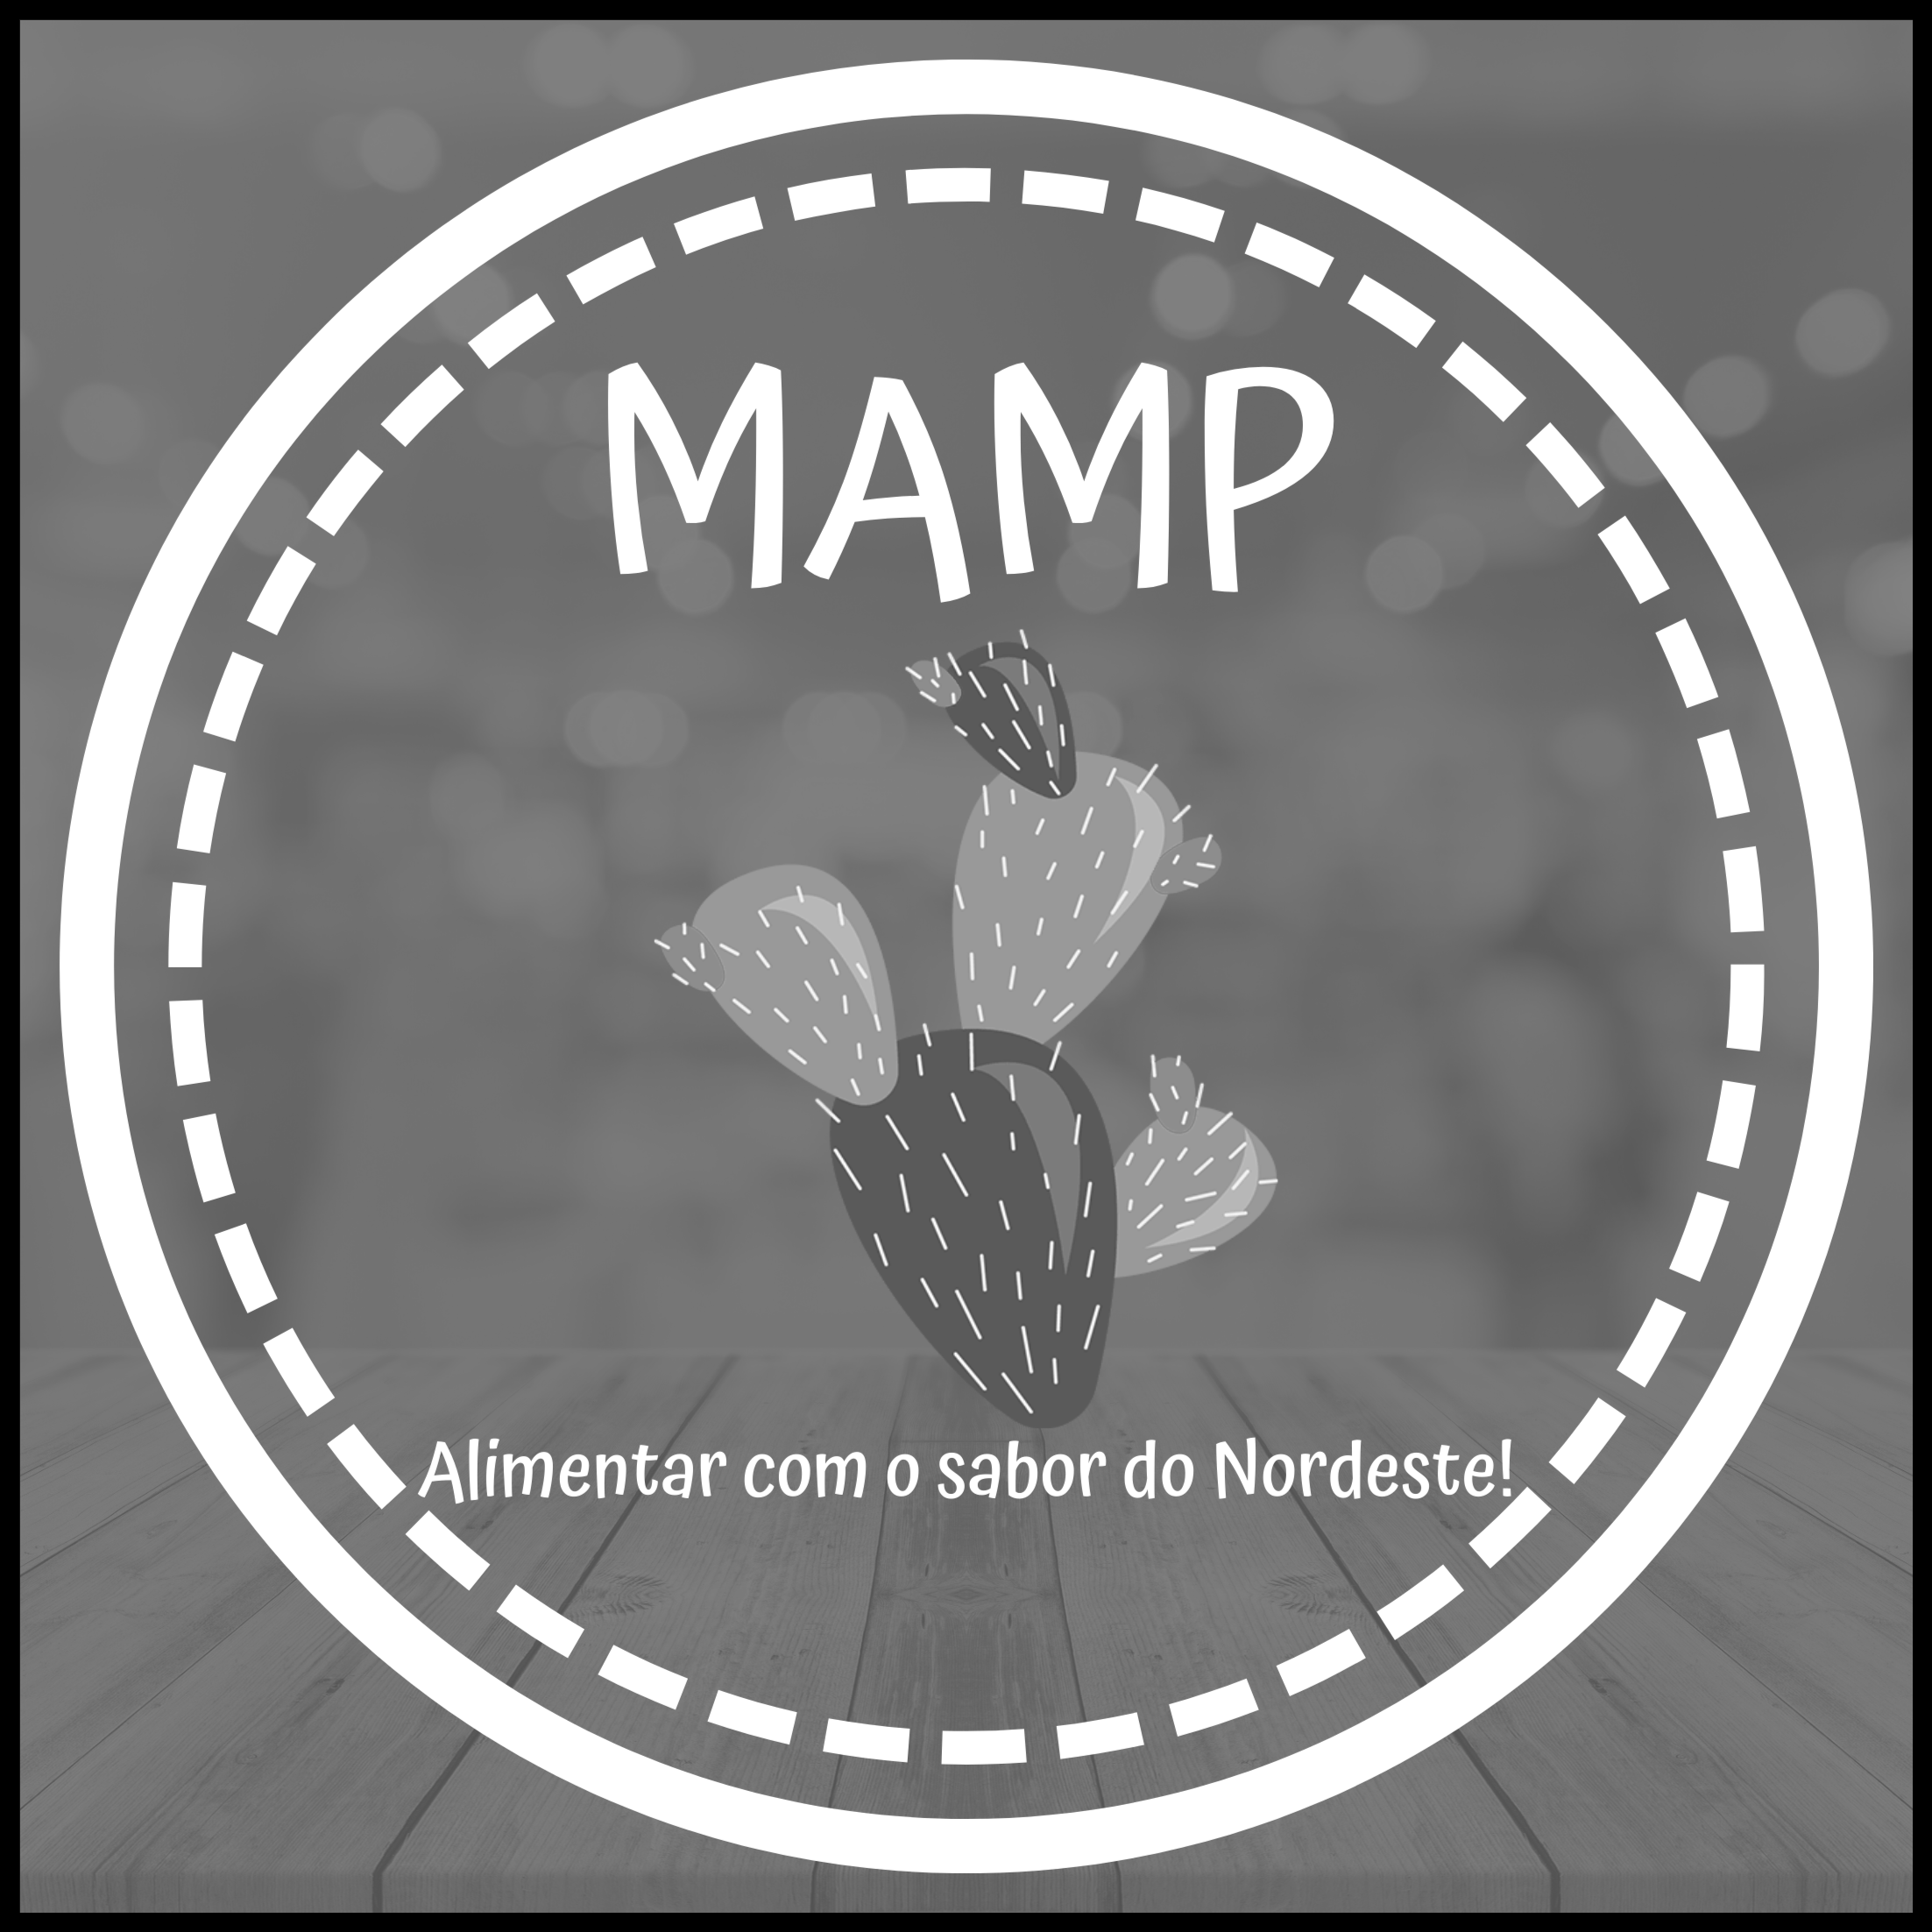
\includegraphics[scale=0.08]{Imagens/mamp.png}
\fonte{\cite{ufs_empreenda_2019}}
\label{figura_22}
\end{figure}



\subsection{Ranagro}

\textbf{PROBLEMA}

O mercado está cada vez mais competitivo, assim sendo necessário uma inovação para alcançar o resultado satisfatório e economicamente viável para o produtor e consumidor, além de trazer tecnologias inovadoras para o ramo da ranicultura. A qualidade e sustentabilidade é vista como uma arma de estratégia para a expansão da empresa. A carne de rã está sendo cada vez mais valorizada e consumida em restaurantes, no qual passou a ser recomendados por médicos e nutricionistas, pois sua taxa de gordura é de apenas três por cento, sendo a única carne produzida em cativeiros que possui dez aminoácidos e indicados também para alimentação de crianças que possuem rejeição à proteína animal, assim, podendo expandir cada vez mais seu consumo. A ração oferecida no mercado é mesma empregada na criação de peixes que acarreta um menor aproveitando da carne e elevando o custo para a engorda.

Assim a Ranagro, veio com uma proposta inovadora para o mercado que é a comercialização de uma ração específica, para haver um menor custo,menor impacto ambiental, crescimento rápido, boa lucratividade e um alto aproveitamento, no qual pode chegar muito próximo a cem por cento, se for considerado a exploração do mercado de subprodutos, como o fígado para pavê e a pele, que atende a medicina humana na recuperação de queimaduras. A ranicultura é uma nova oportunidade para ser explorada no agronegócio e a criação e comercialização da carne de rã, pode ser uma nova forma de ampliar o nicho agrário do país. Nosso grupo é formado por três graduastes de zootecnia e dois de engenharia agronômica, obrigada pela atenção de todos. A marca pode ser vista na Figura \ref{figura_26}), já os produtos podem ser visto no Apêndice \ref{app:workshop_demoday} página 129.



\begin{figure}[H]
\centering
\caption{\textbf{Marca Ranagro}}
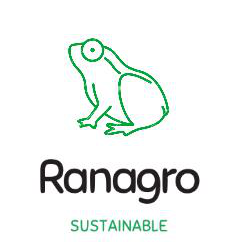
\includegraphics[scale=0.7]{Imagens/ranagro.png}
\fonte{\cite{ufs_empreenda_2019}}
\label{figura_26}
\end{figure}



\subsection{Marca Tecno Coco}

A ideia da Tecno Coco é gerar uma cadeia cíclica de produção onde o Campo produz o coco, que é destinado ao comerciante, vendido ao usuário onde é descartado e processada pela nossa Startup retornando ao Campo como insumo agrícola, auxiliando na produtividade. Outra parte será destinada a outras cadeias produtivas e manufaturas, como material para isolamento acústico, reforço de materiais, enchimento de estofados, mantas para proteção do solo e muitos outros produtos que esse resíduo pode ser transformado. A marca pode ser vista na Figura \ref{figura_50}), já s produtos podem ser visto no Apêndice \ref{app:workshop_demoday} página 124.


\begin{figure}[H]
\centering
\caption{\textbf{Tecno Coco}}
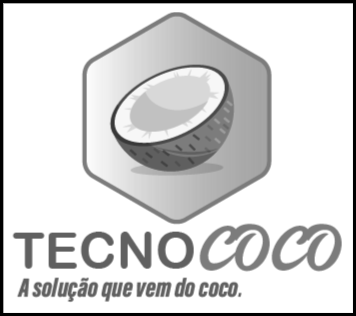
\includegraphics[scale=0.45]{Imagens/tecnococo.png}
\fonte{\cite{ufs_empreenda_2019}}
\label{figura_50}
\end{figure}


\subsection{Une Agro}

Imagine se uma fabrica produzisse uma produto que o único escoamento dele fosse para uma distribuidora na região, essa distribuidora ia ditar preço e quantidade que iria comprar os produtos, podendo até perder a produção. Qual incentivo essa fabrica teria de produzir? Bem isso acontece com diversos agricultores no Brasil, ficam refém apenas de um atravessador que vai até a porta dele para escoar seus produtos, sendo que o atravessador fica com maior parte dos lucros, e muitas vezes o que paga a agricultor é só o custo da produção.

A UneAgro pensando nisso, elaboramos um aplicativo onde o produtor possa anunciar seus produtos de forma pratica e rápida, sem sair de casa, onde ele irá ter uma amplo leque de clientes que estão interessados no produto dele.

O aplicativo é desenvolvido para as duas personas, tanto para agricultor quanto para o distribuidor, pois o distribuidor também sai ganhando ao utilizar o aplicativo pois terá uma maior quantidade localidade e preços pelo mesmo produto, podendo negociar com todas. O aplicativo será totalmente gratuito, sendo que a receita da empresa se originará nas parcerias anunciantes e seus produtos no aplicativo, além de disponibilizar informações produtos que serão disponibilizados para os usuários através de um pacote mensal ou anual, onde esses infoprodutos estarão relacionados ao próprio desenvolvimento de negócio dos usuários, como aulas e \textit{podcasts} sobre gestão e produção agrícola a marca pode ser vista na Figura \ref{figura_28})já os produtos podem ser visto no Apêndice \ref{app:workshop_demoday} página 131.

\begin{figure}[H]
\centering
\caption{\textbf{Marca Une Agro}}

\includegraphics[scale=0.35]{Imagens/uneagro.png}
\fonte{\cite{ufs_empreenda_2019}}
\label{figura_28}
\end{figure}


